\documentclass[12pt,a4paper]{article}

% --- Packages Setup ---
\usepackage[utf8]{inputenc}
\usepackage[indonesian]{babel}
\usepackage[margin=2.5cm,top=2.5cm,bottom=2.5cm,headheight=20pt,headsep=15pt,footskip=25pt]{geometry}
\usepackage{xcolor}
\usepackage{graphicx}
\usepackage{tikz}
\usetikzlibrary{calc}
\usepackage{eso-pic}
\usepackage{fancyhdr}
\usepackage{enumitem}
\usepackage{caption}
\usepackage{tabularx}
\usepackage{colortbl}
\usepackage{booktabs}
\usepackage{hyperref}
\usepackage{titlesec}
\usepackage{mathptmx} % Times New Roman font
\usepackage{amssymb}  % For symbols
\usepackage{setspace} % Line spacing
\usepackage{float}    % For [H] exact float placement
\usepackage{indentfirst} % Indent first paragraph of sections
\usepackage{xurl}     % Better URL line breaking

% --- Line & Paragraph Spacing ---
\setstretch{1.15}
\setlength{\parskip}{4pt}
\setlength{\parindent}{1cm}

% --- Color Definitions (Matching propo-luna.pdf Palette) ---
\definecolor{PrimaryBlue}{HTML}{1E295B}       % Dark Navy Blue for headings
\definecolor{TealAccent}{HTML}{20A090}        % Teal Accent for subheadings, borders & captions
\definecolor{SectionBoxBg}{HTML}{F0F2FA}      % Light Lavender/Blue for section headers
\definecolor{TableHeaderPurple}{HTML}{5B4B9A} % Dark Purple for table header (propo-luna.pdf)
\definecolor{TableAltRowBg}{HTML}{F4F1FB}     % Soft purple background for alternating table rows
\definecolor{TableBorderColor}{HTML}{C4C7C5}  % Soft gray border color for table grid lines
\definecolor{PageFrameColor}{HTML}{E2E8F4}    % Soft frame border color
\definecolor{CalloutBg}{HTML}{EBEFF8}         % Soft background for abstract box

% --- Hyperlink Setup ---
\hypersetup{
    colorlinks=true,
    linkcolor=PrimaryBlue,
    citecolor=TealAccent,
    urlcolor=TealAccent
}

% --- Outer Page Frame Border Setup (Matching propo-luna.pdf) ---
\AddToShipoutPictureBG{%
  \begin{tikzpicture}[overlay,remember picture]
    \draw[line width=0.5pt, PageFrameColor] 
      ($(current page.north west) + (0.9cm,-0.9cm)$) 
      rectangle 
      ($(current page.south east) + (-0.9cm,0.9cm)$);
  \end{tikzpicture}%
}

% --- Header & Footer Setup ---
\pagestyle{fancy}
\fancyhf{}
\lhead{\small\itshape\color{TableHeaderPurple} LUNA -- HOLOGY 9.0}
\rhead{\small\itshape\color{TealAccent} HoloDev Software Development}
\renewcommand{\headrulewidth}{0.5pt}
\renewcommand{\headrule}{\color{TealAccent}\hrule width\headwidth height \headrulewidth}

\cfoot{\small\color{TealAccent} $\blacklozenge$~\thepage~$\blacklozenge$}
\renewcommand{\footrulewidth}{0.5pt}
\renewcommand{\footrule}{\color{TealAccent}\hrule width\headwidth height \footrulewidth}

% --- Custom Section Box Macro (Bulletproof, 100% textwidth) ---
\newcommand{\secbox}[2]{%
  \par\addvspace{1.4em}\noindent
  \begingroup
  \setlength{\fboxsep}{7pt}%
  \colorbox{SectionBoxBg}{%
    \parbox{\dimexpr\textwidth-2\fboxsep\relax}{%
      {\large\bfseries\color{PrimaryBlue} #1\quad #2}%
    }%
  }%
  \par\nointerlineskip
  \vspace{1pt}%
  {\color{TealAccent}\hrule height 2pt width \textwidth}%
  \endgroup
  \par\addvspace{0.7em}\nopagebreak
}

% --- Custom Subsection Macro Bar (Vertically centered green line) ---
\newcommand{\subsecbar}[1]{%
  \par\addvspace{1.0em}\noindent
  \setbox0=\hbox{{\large\bfseries\color{PrimaryBlue} #1}}%
  {\color{TealAccent}\vrule width 3.5pt height \dimexpr\ht0+1pt\relax depth \dimexpr\dp0+1pt\relax}%
  \hspace{6pt}%
  \usebox0%
  \par\addvspace{0.4em}\nopagebreak
}

% --- Custom Lampiran Subheading ---
\newcommand{\lampiranhead}[1]{%
  \par\addvspace{0.9em}\noindent
  {\large\bfseries\color{PrimaryBlue} #1}%
  \par\addvspace{0.4em}\nopagebreak
}

% --- Custom Subsubsection Style ---
\newcommand{\subsubsecstyle}[1]{%
  \par\addvspace{0.5em}\noindent
  {\bfseries\itshape\color{TealAccent} #1}\par\vspace{0.2em}\nopagebreak
}

% --- Abstract / Callout Box Environment ---
\newenvironment{abstractbox}{%
  \par\addvspace{0.8em}\noindent
  \begin{tikzpicture}
    \node[
      fill=CalloutBg,
      draw=TealAccent,
      line width=0.8pt,
      rounded corners=6pt,
      inner xsep=8pt,
      inner ysep=8pt,
      minimum width=\textwidth,
      text width=\dimexpr\textwidth-16pt\relax,
      align=center,
      execute at begin node={\hyphenpenalty=10000\exhyphenpenalty=10000}
    ] \bgroup\itshape\color{PrimaryBlue}%
}{%
    \egroup;
  \end{tikzpicture}%
  \par\addvspace{0.8em}
}

% --- Custom Caption Styling ---
\DeclareCaptionFormat{lunacaption}{%
  \centerline{\small\itshape\color{TealAccent}#1#2#3}%
}
\captionsetup[figure]{format=lunacaption, labelsep=period}
\captionsetup[table]{format=lunacaption, labelsep=period, position=top}

% --- Document Info ---
\title{\textbf{LUNA (Listening, Understanding, Nurturing Assistant)}\\
\large Platform Pendamping Kesehatan Mental Berbasis Multi-Agent Artificial Intelligence dengan Personalized Mental Health Support, Automatic Diary, dan Early Mental Crisis Detection bagi Generasi Z}
\author{Tim Luna AI}
\date{2026}

\begin{document}

% --- Cover Page ---
\begin{titlepage}
\thispagestyle{empty}
\AddToShipoutPictureBG*{
\includegraphics[width=\paperwidth,height=\paperheight]{images/pristine_background_canvas.png}}

\begin{tikzpicture}[remember picture, overlay]
  % --- Logos in Header ---
  % Top Left: POLINEMA Logo
  \node[anchor=north west, inner sep=0pt] at ($(current page.north west) + (2.0cm, -1.8cm)$) {
    
\includegraphics[height=1.8cm, keepaspectratio]{images/logo_polinema.png}
  };
  
  % Top Right: HOLOGY 9.0 White Logo
  \node[anchor=north east, inner sep=0pt] at ($(current page.north east) + (-2.0cm, -1.8cm)$) {
    
\includegraphics[height=1.8cm, keepaspectratio]{images/logo-hology-white.png}
  };

  % --- Category Tagline ---
  \node[anchor=north, align=center] at ($(current page.north) + (0cm, -4.0cm)$) {
    {\fontfamily{phv}\selectfont\sffamily\bfseries\color{PrimaryBlue}\small PROPOSAL SOFTWARE DEVELOPMENT \hspace{4pt}$\bullet$\hspace{4pt} HOLOGY 9.0}
  };

  % --- Main Title: LUNA ---
  \node[anchor=north, align=center] at ($(current page.north) + (0cm, -7.0cm)$) {
    {\fontfamily{phv}\selectfont\sffamily\bfseries\color{PrimaryBlue}\fontsize{42pt}{48pt}\selectfont LUNA}\\[8pt]
    {\fontfamily{phv}\selectfont\sffamily\bfseries\itshape\color{TealAccent}\fontsize{14pt}{18pt}\selectfont (Listening, Understanding, Nurturing Assistant)}
  };

  % --- Subtitle / Description ---
  \node[anchor=north, align=center, text width=16.0cm, execute at begin node={\hyphenpenalty=10000\exhyphenpenalty=10000}] at ($(current page.north) + (0cm, -10.2cm)$) {
    {\fontfamily{phv}\selectfont\sffamily\bfseries\color{PrimaryBlue}\fontsize{11.5pt}{17.5pt}\selectfont Platform Pendamping Kesehatan Mental Berbasis \textit{Multi-Agent Artificial Intelligence} dengan \textit{Personalized Mental Health Support}, \textit{Automatic Diary}, dan \textit{Early Mental Crisis Detection} bagi Generasi Z}
  };

  % --- Team & University Info at Bottom ---
  \node[anchor=south, align=center] at ($(current page.south) + (0cm, 2.5cm)$) {
    {\fontfamily{phv}\selectfont\sffamily\bfseries\color{PrimaryBlue}\fontsize{14pt}{18pt}\selectfont TIM LUNA AI}\\[5pt]
    {\fontfamily{phv}\selectfont\sffamily\bfseries\color{TealAccent}\fontsize{12pt}{16pt}\selectfont POLITEKNIK NEGERI MALANG}\\[4pt]
    {\fontfamily{phv}\selectfont\sffamily\color{PrimaryBlue!80}\fontsize{11pt}{14pt}\selectfont 2026}
  };
\end{tikzpicture}

\null
\end{titlepage}

\newpage

% --- Main Sections Import ---
% === I. Judul / Nama Perangkat Lunak ===
\secbox{I.}{Judul / Nama Perangkat Lunak}

\begin{abstractbox}
\centering
\textbf{LUNA (Listening, Understanding, Nurturing Assistant): Platform Pendamping Kesehatan Mental Berbasis Multi-Agent Artificial Intelligence dengan Personalized Mental Health Support, Automatic Diary, dan Early Mental Crisis Detection bagi Generasi Z}
\end{abstractbox}

\indent
\textbf{LUNA (Listening, Understanding, Nurturing Assistant)} merupakan platform pendamping kesehatan mental berbasis \textit{Multi-Agent Artificial Intelligence} yang dirancang untuk memberikan dukungan kesehatan mental secara personal bagi Generasi Z. Nama LUNA sendiri merepresentasikan kemampuan sistem dalam mendengarkan (\textit{listening}), memahami kondisi emosional pengguna (\textit{understanding}), memberikan dukungan yang adaptif (\textit{nurturing}), serta berperan sebagai asisten digital (\textit{assistant}) yang siap mendampingi pengguna melalui percakapan berbasis teks maupun suara.

Selain itu, LUNA mengintegrasikan beberapa agen kecerdasan buatan yang bekerja secara kolaboratif untuk menyediakan \textit{Personalized Mental Health Support}, menyusun \textit{Automatic Diary} berdasarkan hasil percakapan, serta melakukan \textit{Early Mental Crisis Detection} sebagai upaya deteksi dini terhadap potensi krisis kesehatan mental.

\vspace{0.5em}
\begin{abstractbox}
\centering
\textbf{Tautan Akses Berkas, Source Code, \& Video Demo Perangkat Lunak:}\\[0.3em]
\small
\url{https://drive.google.com/drive/folders/1bJp6CdtFBXfh3RJ8tv2wlBQT3z1xdhio?usp=drive_link}\\[0.2em]
{\small\itshape (Folder Google Drive berisi Berkas Source Code, Build APK, Dokumentasi Teknis, dan Video Demo Aplikasi LUNA)}
\end{abstractbox}

% === II. Latar Belakang Ide Perangkat Lunak ===
\secbox{II.}{Latar Belakang Ide Perangkat Lunak}

Krisis kesehatan mental telah menjadi isu kesehatan publik global, dengan hampir 1,1 miliar jiwa (1 dari 7 orang) hidup dengan gangguan psikologis, termasuk gangguan kecemasan dan depresi (Dhia Tawakalna \& Junta Zeniarja, 2026; Gong et al., 2026). Seperti yang terlihat pada Gambar 1, sekitar 9,8\% penduduk di Indonesia mengalami gangguan psikologis, namun hanya 2,5\% yang memperoleh layanan konseling profesional akibat rendahnya literasi kesehatan mental (Dhia Tawakalna \& Junta Zeniarja, 2026). Kondisi ini secara signifikan memengaruhi Generasi Z (10--24 tahun), yang merupakan periode munculnya sekitar 75\% gangguan mental pertama kali (Casey Annie E., 2024). Berbagai studi juga menunjukkan bahwa 84\% Generasi Z menganggap kesehatan mental sebagai krisis nasional, 91\% pernah mengalami stres, sementara 60\% merasa kewalahan menghadapi berbagai tekanan global, tetapi hanya separuh yang mengetahui tempat memperoleh bantuan psikologis (Arrahmi Thahir et al., 2023; Casey Annie E., 2024, 2025; UNICEF, 2025).

\begin{figure}[H]
    \centering
    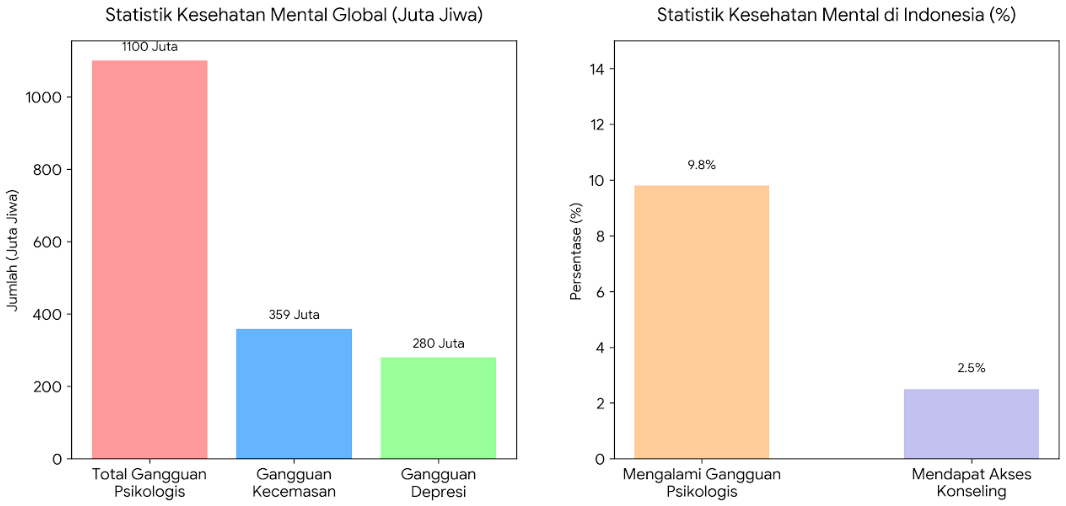
\includegraphics[width=0.85\textwidth]{images/bab2/fig1_statistik.png}
    \caption{Statistik Kesehatan Mental}
\end{figure}

Kerentanan tersebut dipengaruhi oleh penggunaan internet dan media sosial secara intensif yang memicu isolasi sosial, kesepian, gangguan tidur, perundungan siber, serta fenomena \textit{Fear of Missing Out} (FOMO), dan diperparah oleh tekanan ekonomi, akademik, kecemasan iklim, hingga kekhawatiran terhadap otomatisasi pekerjaan oleh kecerdasan buatan (Arrahmi Thahir et al., 2023; Fadli, 2024). Tanpa intervensi dini, kondisi ini berdampak pada penurunan konsentrasi belajar, penarikan diri dari lingkungan sosial, serta peningkatan risiko bunuh diri yang menjadi salah satu penyebab utama kematian pada kelompok usia 15--29 tahun (Arrahmi Thahir et al., 2023; Casey Annie E., 2025; Fadli, 2024).

Meskipun kebutuhan akan pendampingan psikologis semakin mendesak, akses terhadap layanan profesional masih terhambat oleh keterbatasan jumlah psikolog, tingginya biaya terapi, serta stigma sosial terhadap pencari bantuan (Arrahmi Thahir et al., 2023; Dhia Tawakalna \& Junta Zeniarja, 2026). Di sisi lain, aplikasi kesehatan mental berbasis aturan (\textit{rule-based}) belum mampu memahami percakapan secara empatik (Dhia Tawakalna \& Junta Zeniarja, 2026). Sementara itu, pemanfaatan Large Language Model (LLM) generatif tunggal berisiko memicu halusinasi medis (Fransson, 2026), tidak memiliki memori percakapan jangka panjang antar-sesi (Packer et al., 2024), serta membebankan pencatatan diari secara manual yang sering diabaikan pengguna. Tinjauan literatur juga menunjukkan adanya kesenjangan keselamatan (\textit{safety gap}), di mana 48,28\% chatbot kesehatan mental komersial gagal memberikan respons yang memadai terhadap situasi krisis bunuh diri (Elbarbary et al., 2026).

Guna memastikan keabsahan ilmiah dan efektivitas dalam mengukur kondisi emosional pengguna, tim pengembang telah melakukan studi pendahuluan dan wawancara klinis bersama \textbf{Qori Fanani, M.Psi., Psikolog} (Petugas Poliklinik Politeknik Negeri Malang dan Dosen Psikologi Universitas Kepanjen). Berdasarkan hasil konsultasi tersebut, instrumen \textbf{DASS-21 (\textit{Depression Anxiety Stress Scale 21})} direkomendasikan dan divalidasi sebagai kerangka kerja psikometris utama dalam LUNA. Kerangka DASS-21 memungkinkan sistem mengukur tiga indikator psikologis utama—yaitu tingkat depresi, kecemasan (\textit{anxiety}), dan stres—secara terpisah melalui perhitungan skor yang terukur, sehingga LUNA mampu membedakan tingkat distres emosional non-klinis secara akurat (Dokumentasi wawancara disajikan pada Lampiran 6).

Berdasarkan permasalahan tersebut, penulis mengusulkan LUNA (Listening, Understanding, Nurturing Assistant) sebagai platform pendamping kesehatan mental berbasis Multi-Agent AI bagi Generasi Z yang mengintegrasikan enam fitur utama, yaitu \textit{Personalized Mental Health Support}, \textit{Automatic Diary Generation}, \textit{Long-term Conversation Memory}, \textit{Emotion \& Mental Risk Analysis}, \textit{Early Mental Crisis Detection}, dan \textit{Voice Conversation}. Kebaruan LUNA terletak pada arsitektur Multi-Agent AI yang mengorkestrasi agen terapis, pembuat diari, penilai risiko krisis, dan pengelola memori berbasis RAG, sehingga mampu memberikan pendampingan yang lebih personal, berkelanjutan, dan aman dibandingkan chatbot berbasis LLM tunggal. LUNA selaras dengan subtema AI in Health and Well-being AI untuk meningkatkan akses pendampingan psikologis awal dan deteksi dini krisis emosional.

% === III. Tujuan dan Manfaat Dikembangkannya Perangkat Lunak ===
\secbox{III.}{Tujuan dan Manfaat Dikembangkannya Perangkat Lunak}

\subsecbar{3.1 Tujuan Pengembangan Perangkat Lunak}
Secara khusus, tujuan pengembangan LUNA meliputi:
\begin{enumerate}[leftmargin=*,label=\arabic*.]
    \item Menyediakan layanan pendampingan psikologis awal yang dapat diakses kapan saja.
    \item Menghasilkan diari emosional secara otomatis melalui \textit{Automatic Diary Generation}.
    \item Mempertahankan konteks percakapan antar-sesi menggunakan \textit{Long-term Conversation Memory}.
    \item Mendeteksi dini risiko krisis emosional melalui \textit{Early Mental Crisis Detection}.
    \item Menyediakan interaksi suara yang natural melalui fitur \textit{Voice Conversation}.
\end{enumerate}

\subsecbar{3.2 Manfaat Pengembangan Perangkat Lunak}

\subsubsecstyle{Bagi Pengguna (Generasi Z)}
\begin{enumerate}[leftmargin=*,label=\arabic*.]
    \item Menyediakan ruang aman untuk mengekspresikan kondisi emosional.
    \item Membantu mengenali pola emosi dan melakukan refleksi diri.
    \item Memberikan pendampingan psikologis yang lebih personal dan berkelanjutan.
\end{enumerate}

\subsubsecstyle{Bagi Masyarakat}
\begin{enumerate}[leftmargin=*,label=\arabic*.]
    \item Mendukung deteksi dini dan pencegahan krisis kesehatan mental.
    \item Meningkatkan literasi kesehatan mental serta mengurangi stigma.
    \item Memperluas akses pendampingan psikologis awal, terutama bagi masyarakat dengan keterbatasan layanan profesional.
\end{enumerate}

\subsubsecstyle{Bagi Pengembangan AI di Bidang Kesehatan}
\begin{enumerate}[leftmargin=*,label=\arabic*.]
    \item Mengimplementasikan arsitektur Multi-Agent AI untuk pendampingan kesehatan mental.
    \item Memanfaatkan Retrieval-Augmented Generation (RAG) guna meningkatkan akurasi dan mengurangi halusinasi informasi.
    \item Mendukung pengembangan AI yang lebih aman melalui mekanisme deteksi krisis dan AI Safety Guardrails.
\end{enumerate}

% === IV. Batasan Perangkat Lunak ===
\secbox{IV.}{Batasan Perangkat Lunak}

Pengembangan perangkat lunak LUNA dibatasi pada ketentuan-ketentuan yang disajikan pada Tabel 1.

\begin{table}[H]
\centering
\renewcommand{\arraystretch}{1.35}
\renewcommand{\tabularxcolumn}[1]{m{#1}}
\arrayrulecolor{TableBorderColor}
\caption{Batasan Perangkat Lunak}
\vspace{0.3em}
\small
\begin{tabularx}{\textwidth}{| c | >{\bfseries}l | X |}
\hline
\rowcolor{TableHeaderPurple}
\color{white}\bfseries No & \color{white}\bfseries Aspek Batasan & \color{white}\bfseries Deskripsi Batasan \\
\hline
1 & Cakupan Pengguna & Ditujukan bagi Generasi Z sebagai pendamping psikologis awal (\textit{digital first-aid}), bukan untuk penanganan gangguan jiwa berat atau kondisi krisis akut. \\
\hline
\rowcolor{TableAltRowBg}
2 & Fungsi Utama & Mendukung \textit{Personalized Support}, \textit{Automatic Diary}, \textit{Long-term Memory}, \textit{Emotion Analysis}, \textit{Crisis Detection}, \textit{Therapy Recommendation}, dan \textit{Voice Conversation}. \\
\hline
3 & Platform & Tersedia pada aplikasi mobile. \\
\hline
\rowcolor{TableAltRowBg}
4 & Teknologi & Menggunakan Multi-Agent AI, DeepSeek LLM, RAG, Long-term Memory, Speech-to-Text, dan Text-to-Speech. \\
\hline
5 & Kemampuan AI & Berfungsi sebagai pendamping digital dan tidak memberikan diagnosis medis maupun menggantikan psikolog atau psikiater. \\
\hline
\rowcolor{TableAltRowBg}
6 & Data \& Penyimpanan & Data percakapan dienkripsi dan dianonimkan, sedangkan basis pengetahuan RAG berasal dari literatur psikologi terverifikasi. \\
\hline
7 & Deteksi Krisis & Mendeteksi risiko krisis melalui analisis teks dan emosi, kemudian mengarahkan pengguna ke hotline atau layanan profesional jika diperlukan. \\
\hline
\rowcolor{TableAltRowBg}
8 & Etika \& Operasional & Menerapkan AI Safety Guardrails untuk menolak respons berbahaya; performa fitur suara bergantung pada perangkat dan kualitas masukan pengguna. \\
\hline
\end{tabularx}
\end{table}

% === V. Metodologi Pengembangan Perangkat Lunak ===
\secbox{V.}{Metodologi Pengembangan Perangkat Lunak}

Pengembangan perangkat lunak menggunakan metode \textit{Agile Software Development} karena mendukung proses yang iteratif, adaptif, dan fleksibel terhadap perubahan kebutuhan. Melalui pendekatan ini, setiap fitur dapat dikembangkan, diuji, dan dievaluasi secara bertahap untuk meningkatkan kualitas sistem. Tahapan pengembangan LUNA ditunjukkan pada Gambar 2.

\begin{figure}[H]
    \centering
    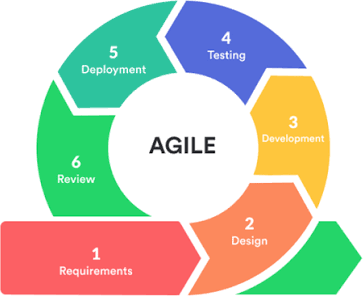
\includegraphics[width=0.50\textwidth]{images/bab5/fig2_agile.png}
    \caption{Tahapan Agile}
\end{figure}

\subsecbar{1. Requirements}
Tahap Requirements bertujuan mengidentifikasi kebutuhan sistem berdasarkan studi literatur, analisis permasalahan kesehatan mental Generasi Z, serta kebutuhan pengguna terhadap layanan pendamping kesehatan mental digital. Pada tahap ini dilakukan analisis kebutuhan fungsional dan nonfungsional sistem, penentuan fitur utama, serta penyusunan spesifikasi perangkat lunak sebagai dasar proses pengembangan.

\subsecbar{2. Design}
Tahap Design dilakukan untuk merancang solusi perangkat lunak berdasarkan kebutuhan yang telah diperoleh. Perancangan meliputi arsitektur sistem, desain basis data, desain antarmuka pengguna (\textit{User Interface}), serta perancangan arsitektur Multi-Agent Artificial Intelligence yang mengoordinasikan berbagai agen AI untuk menjalankan fungsi pendampingan kesehatan mental, analisis risiko, penyusunan diary otomatis, dan pengelolaan memori percakapan.

\subsecbar{3. Development}
Pada tahap Development, seluruh rancangan diimplementasikan menjadi perangkat lunak yang dapat dijalankan. Pengembangan dilakukan secara bertahap dengan membangun setiap modul utama LUNA, seperti \textit{Personalized Mental Health Support}, \textit{Automatic Diary}, \textit{Long-term Memory}, \textit{Mental Risk Assessment}, \textit{Early Mental Crisis Detection}, serta \textit{Voice Conversation}, kemudian mengintegrasikannya menjadi satu kesatuan sistem.

\subsecbar{4. Testing}
Tahap Testing bertujuan memastikan setiap fitur berjalan sesuai dengan kebutuhan sistem. Pengujian dilakukan terhadap fungsi-fungsi utama, integrasi antar modul, serta alur penggunaan aplikasi untuk memastikan sistem mampu memberikan layanan yang stabil, akurat, dan sesuai dengan rancangan.

\subsecbar{5. Deployment}
Tahap Deployment merupakan proses implementasi perangkat lunak sehingga dapat digunakan oleh pengguna. Pada tahap ini aplikasi dipublikasikan pada lingkungan operasional, dilakukan konfigurasi layanan pendukung, serta memastikan seluruh komponen sistem dapat beroperasi dengan baik.

\subsecbar{6. Review}
Tahap Review dilakukan sebagai proses evaluasi terhadap hasil pengembangan berdasarkan pengujian dan umpan balik pengguna. Hasil evaluasi digunakan sebagai dasar penyempurnaan fitur, peningkatan performa sistem, serta perencanaan iterasi pengembangan berikutnya sehingga LUNA dapat terus berkembang sesuai kebutuhan pengguna.

% === VI. Analisis Kebutuhan dan Desain Solusi Perangkat Lunak ===
\secbox{VI.}{Analisis Kebutuhan dan Desain Solusi Perangkat Lunak}

\subsecbar{6.1 Analisis Kebutuhan}
Berdasarkan hasil identifikasi kebutuhan pengguna dan studi literatur, kebutuhan perangkat lunak LUNA dibagi menjadi dua kategori, yaitu kebutuhan fungsional dan kebutuhan nonfungsional.

\subsubsecstyle{1. Kebutuhan fungsional}
\begin{enumerate}[leftmargin=*,label=\alph*.]
    \item Menyediakan dialog empatik yang terpersonalisasi sesuai profil dan kondisi emosional pengguna.
    \item Menghasilkan \textit{Automatic Diary Generation} dari hasil percakapan.
    \item Mengelola \textit{Long-term Conversation Memory} untuk menyimpan dan memanggil kembali informasi penting pengguna.
    \item Melakukan analisis emosi dan sentimen secara \textit{real-time}.
    \item Mendeteksi krisis emosional serta mengaktifkan protokol penanganan dan rekomendasi bantuan darurat.
    \item Memberikan rekomendasi latihan relaksasi, teknik CBT mandiri, dan materi psikoedukasi berbasis bukti klinis.
    \item Mendukung komunikasi suara melalui \textit{Speech-to-Text} dan \textit{Text-to-Speech}.
\end{enumerate}

\subsubsecstyle{2. Kebutuhan nonfungsional}
\begin{enumerate}[leftmargin=*,label=\alph*.]
    \item Menjamin keamanan data melalui enkripsi dan anonimisasi informasi pribadi.
    \item Menggunakan \textit{Retrieval-Augmented Generation} (RAG) berbasis literatur klinis untuk meningkatkan akurasi respons dan meminimalkan halusinasi.
    \item Menyediakan waktu respons yang cepat untuk percakapan teks maupun suara secara \textit{real-time}.
    \item Menyajikan antarmuka yang intuitif, nyaman, dan mudah digunakan oleh Generasi Z.
\end{enumerate}

\subsecbar{6.2 Desain Solusi}
Desain solusi LUNA disusun untuk menggambarkan konsep, arsitektur, dan mekanisme kerja sistem dalam mewujudkan layanan pendamping kesehatan mental berbasis Multi-Agent Artificial Intelligence. Bagian ini menjelaskan rancangan solusi yang menjadi dasar pengembangan perangkat lunak secara terstruktur.

\subsubsecstyle{1. Gambaran solusi}
\begin{figure}[H]
    \centering
    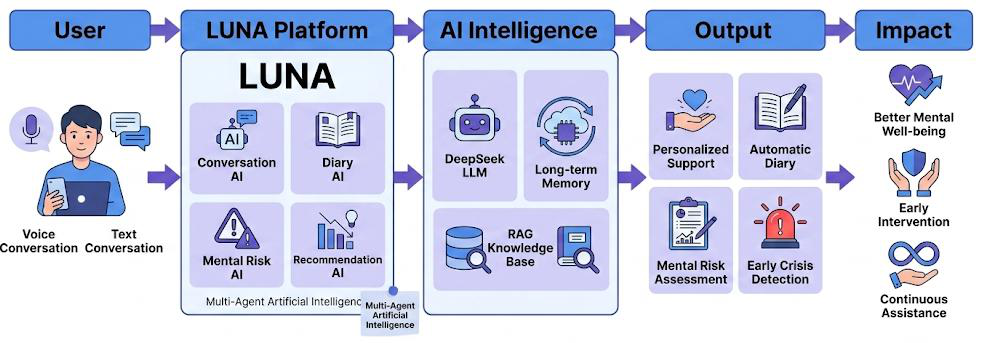
\includegraphics[width=0.80\textwidth]{images/bab6/fig3_konsep.png}
    \caption{Gambaran Konsep LUNA}
\end{figure}

\subsubsecstyle{2. Kerangka Evaluasi Risiko \& Integrasi DASS-21}
Dalam mengevaluasi kondisi emosional pengguna, LUNA mengintegrasikan instrumen psikometris \textbf{DASS-21 (\textit{Depression Anxiety Stress Scale 21})} yang divalidasi oleh pakar psikologi. DASS-21 mengevaluasi tiga subskala emosional utama:
\begin{enumerate}[leftmargin=*,label=\arabic*.]
    \item \textbf{Subskala Depresi}: Mengukur tingkat keputusasaan, devaluasi diri, dan hilangnya minat (7 butir pertanyaan).
    \item \textbf{Subskala Kecemasan (\textit{Anxiety})}: Mengukur respons gairah otonom, efek fisiologis, dan kecemasan situasional (7 butir pertanyaan).
    \item \textbf{Subskala Stres}: Mengukur ketegangan persisten, iritabilitas, dan kesulitan bersantai (7 butir pertanyaan).
\end{enumerate}

Perhitungan skor pada masing-masing subskala dilakukan dengan menjumlahkan nilai butir (skala 0--3) lalu dikalikan 2 ($\mathrm{Skor} = \mathrm{Total\ Subskala} \times 2$). Berdasarkan norma psikometris DASS-21, skor tersebut dikelompokkan ke dalam tiga tingkatan level distres emosional:
\begin{itemize}[leftmargin=*]
    \item \textbf{Level 1 (Tingkat Ringan / \textit{Mild})}: Pengguna mengalami distres emosional ringan. LUNA memberikan psikoedukasi, validasi emosi, dan latihan relaksasi mandiri.
    \item \textbf{Level 2 (Tingkat Sedang / \textit{Moderate})}: Pengguna mengalami distres emosional sedang. LUNA mengaktifkan pendampingan CBT interaktif, penelusuran diari emosional, dan rekomendasi aktivitas terstruktur.
    \item \textbf{Level 3 (Tingkat Berat / \textit{Severe} -- \textit{Extremely Severe})}: Pengguna mengalami distres emosional tinggi atau indikasi krisis. Sistem \textit{RiskAssessmentService} secara otomatis memicu protokol \textit{Safety Gate} untuk memberikan modul bantuan darurat dan rujukan ke kontak profesional/hotline.
\end{itemize}

Hasil penilaian DASS-21 diteruskan ke komponen backend \textit{RiskAssessmentService} untuk menentukan strategi pendampingan yang tepat tanpa melakukan diagnosis medis formal.

\clearpage
\subsubsecstyle{3. Arsitektur sistem}
\begin{figure}[H]
    \centering
    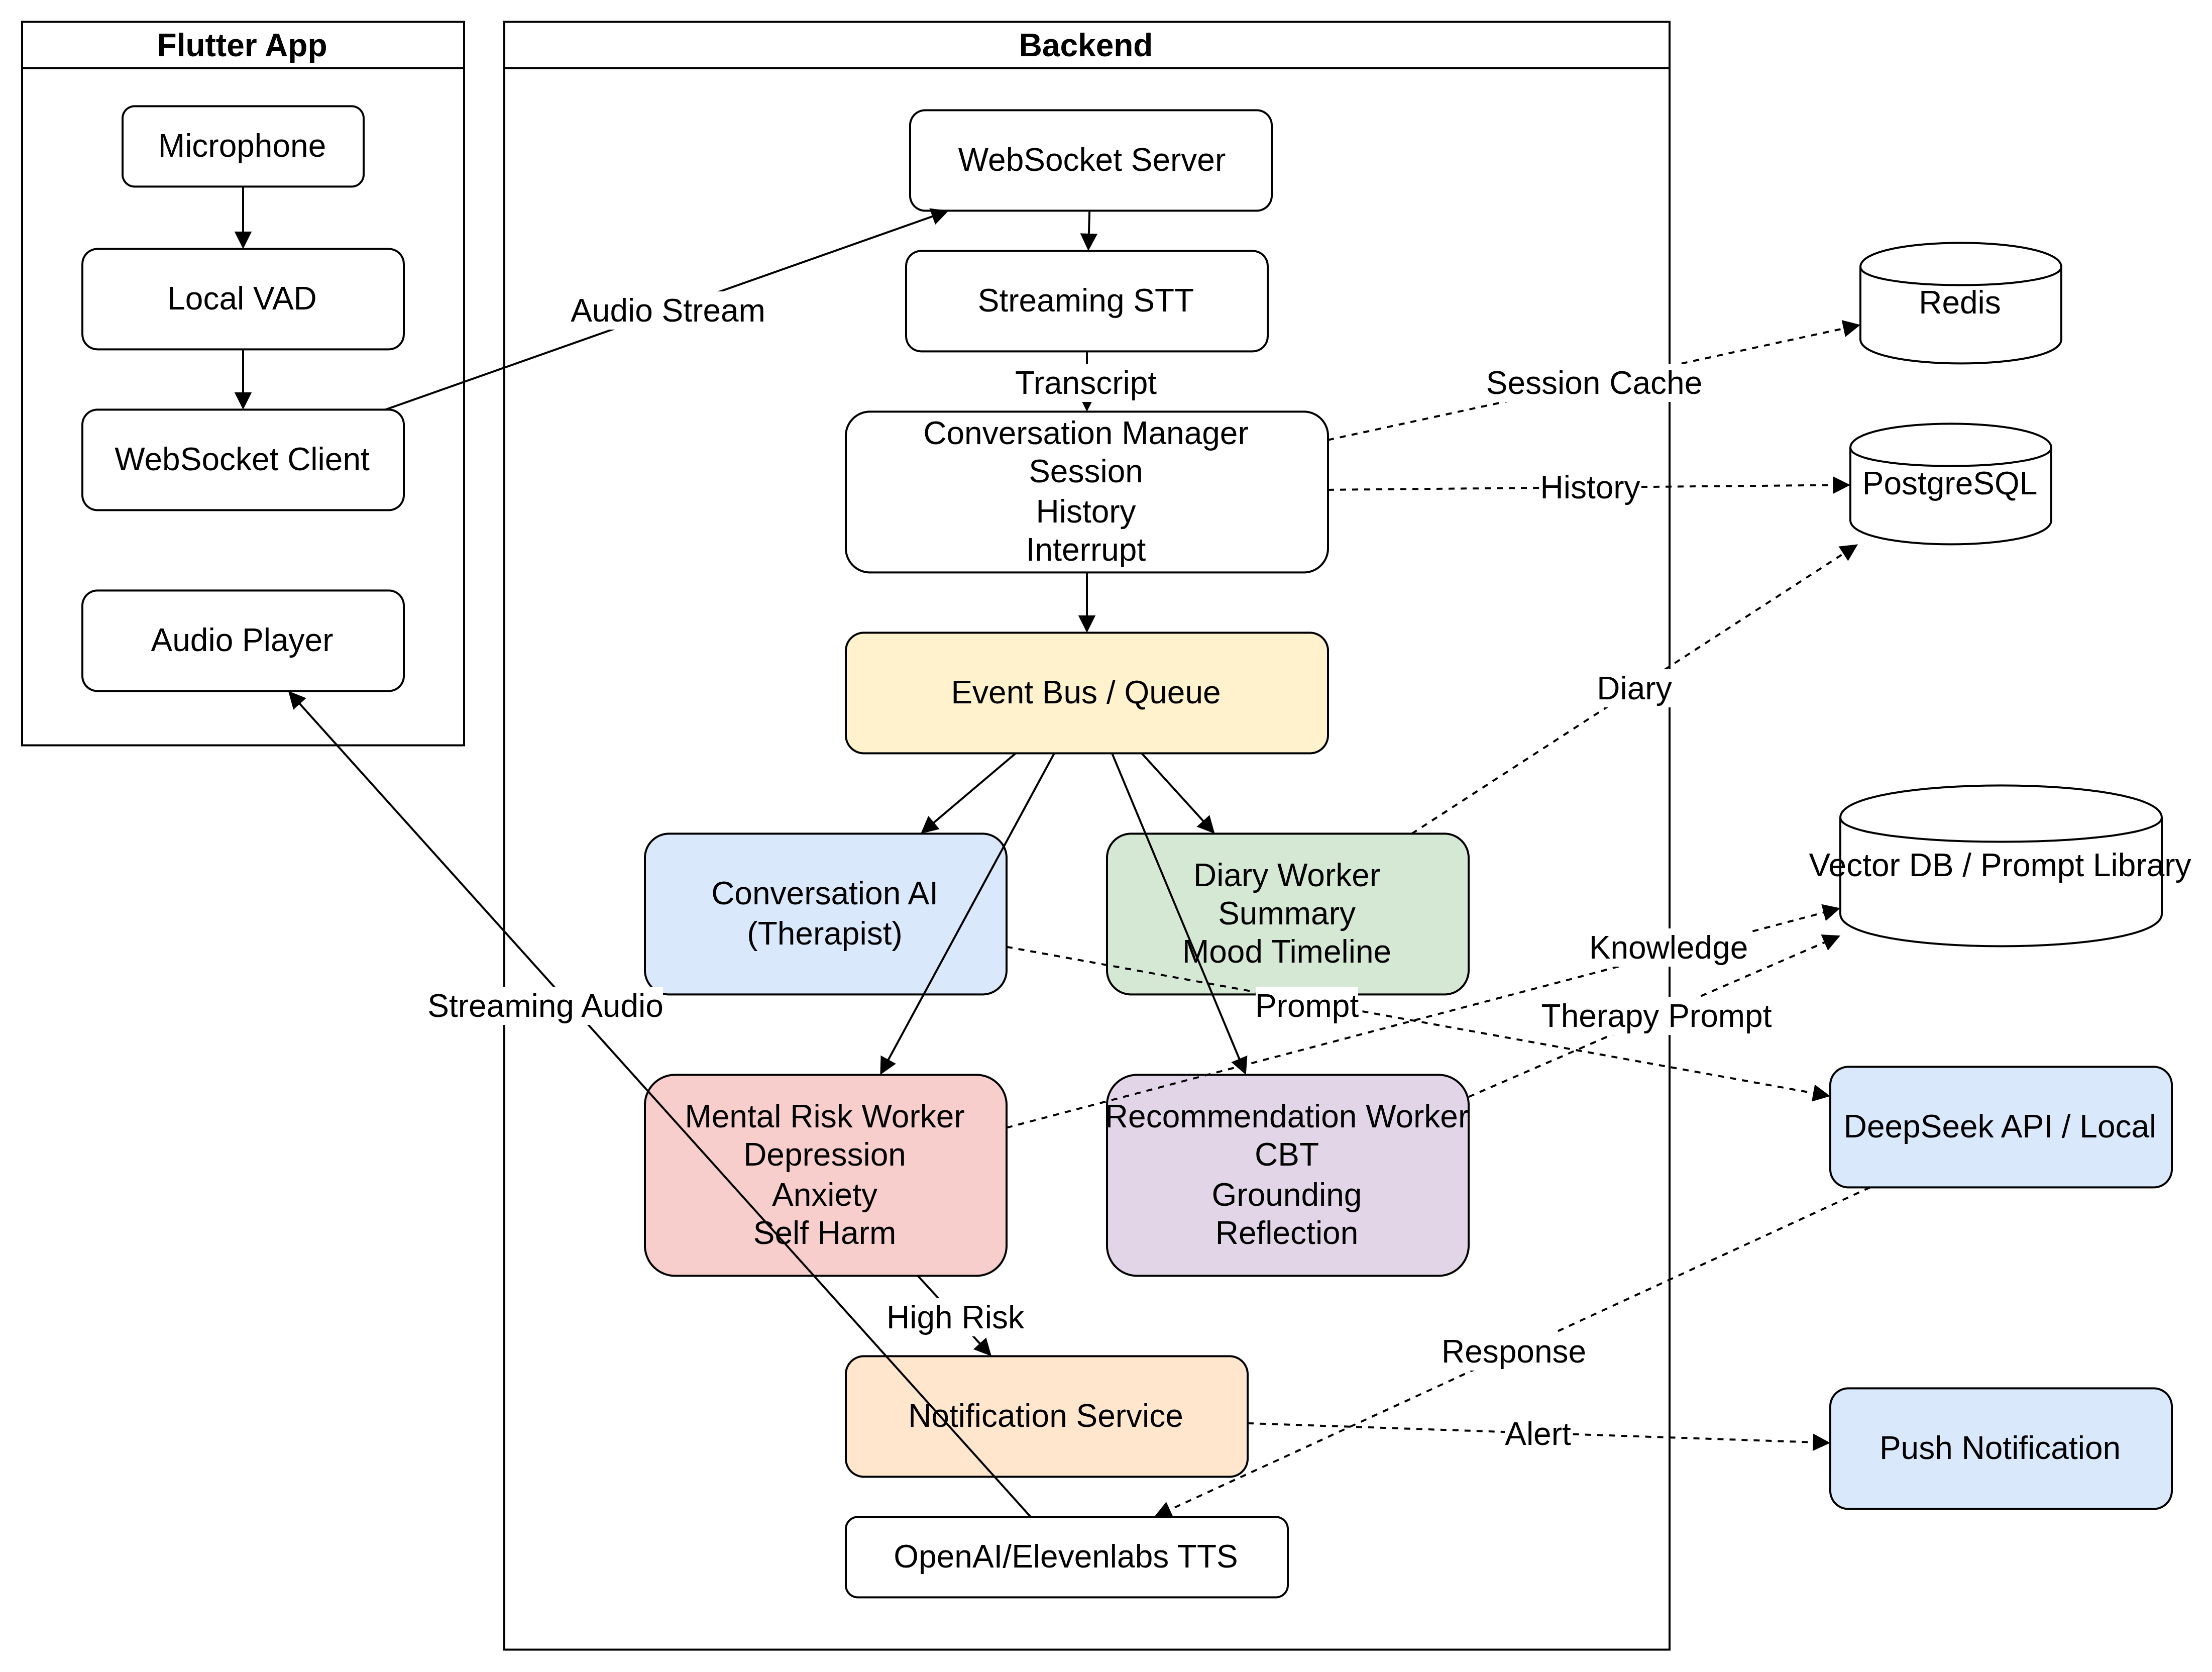
\includegraphics[width=0.85\textwidth]{images/bab6/fig4_arsitektur.png}
    \caption{Arsitektur LUNA}
\end{figure}

% === VII. Implementasi Perangkat Lunak ===
\secbox{VII.}{Implementasi Perangkat Lunak}

\subsecbar{7.1 Implementasi Teknologi}
Implementasi LUNA memanfaatkan kombinasi teknologi modern untuk mendukung komunikasi \textit{real-time}, pemrosesan kecerdasan buatan, penyimpanan data, serta pengalaman pengguna yang responsif. Rincian teknologi yang digunakan ditunjukkan pada Tabel 2.

\begin{table}[H]
\centering
\renewcommand{\arraystretch}{1.35}
\renewcommand{\tabularxcolumn}[1]{m{#1}}
\arrayrulecolor{TableBorderColor}
\caption{Implementasi Teknologi LUNA}
\vspace{0.3em}
\small
\begin{tabularx}{\textwidth}{| >{\bfseries\itshape}l | X |}
\hline
\rowcolor{TableHeaderPurple}
\color{white}\bfseries Komponen & \color{white}\bfseries Fungsi \\
\hline
Mobile Application (Flutter) & Pengembangan aplikasi Android dan iOS \\
\hline
\rowcolor{TableAltRowBg}
Backend Service (FastAPI) & REST API, WebSocket, dan orkestrasi Multi-Agent AI \\
\hline
Artificial Intelligence (DeepSeek LLM) & Menghasilkan respons percakapan yang natural dan kontekstual \\
\hline
\rowcolor{TableAltRowBg}
Speech-to-Text (OpenAI STT) & Mengubah suara menjadi teks \\
\hline
Text-to-Speech (OpenAI TTS) & Menghasilkan respons suara yang natural \\
\hline
\rowcolor{TableAltRowBg}
AI Architecture (Multi-Agent AI) & Mengelola kolaborasi antar agen AI \\
\hline
Knowledge Retrieval (RAG) & Mengambil referensi kesehatan mental yang relevan \\
\hline
\rowcolor{TableAltRowBg}
Vector Database (Qdrant) & Penyimpanan embedding dan pencarian semantik \\
\hline
Database (PostgreSQL) & Penyimpanan data pengguna, diary, dan riwayat percakapan \\
\hline
\rowcolor{TableAltRowBg}
Cache (Redis) & Penyimpanan sesi dan cache percakapan \\
\hline
Long-term Memory (Memory Worker) & Menyimpan preferensi dan konteks pengguna \\
\hline
\end{tabularx}
\end{table}

\subsecbar{7.2 Alur Penggunaan Sistem}
Alur penggunaan LUNA menjelaskan proses interaksi end-to-end antara pengguna dan sistem dalam memanfaatkan seluruh fitur utama. Secara rinci, alur operasional terdiri dari empat tahapan utama:
\begin{enumerate}[leftmargin=*,label=\arabic*.]
    \item \textbf{Autentikasi \& Onboarding}: Pengguna melakukan registrasi/login dan menyetujui etika layanan serta \textit{medical disclaimer}.
    \item \textbf{Dashboard \& Mood Monitoring}: Pengguna mencatat emosi harian (\textit{mood tracker}) dan memantau perkembangan tren kondisi emosional.
    \item \textbf{Konseling Interaktif (Teks \& Suara)}: Pengguna berinteraksi dalam sesi percakapan real-time dengan agen AI berbasis CBT.
    \item \textbf{Sintesis Jurnal \& Safety Gates}: Sistem backend secara otomatis merangkum jurnal harian, memantau tingkat risiko emosional, serta memicu intervensi darurat jika terdeteksi situasi krisis (\textit{High Risk}).
\end{enumerate}

Rangkaian alur penggunaan sistem tersebut disajikan pada Gambar 5.

\begin{figure}[H]
    \centering
    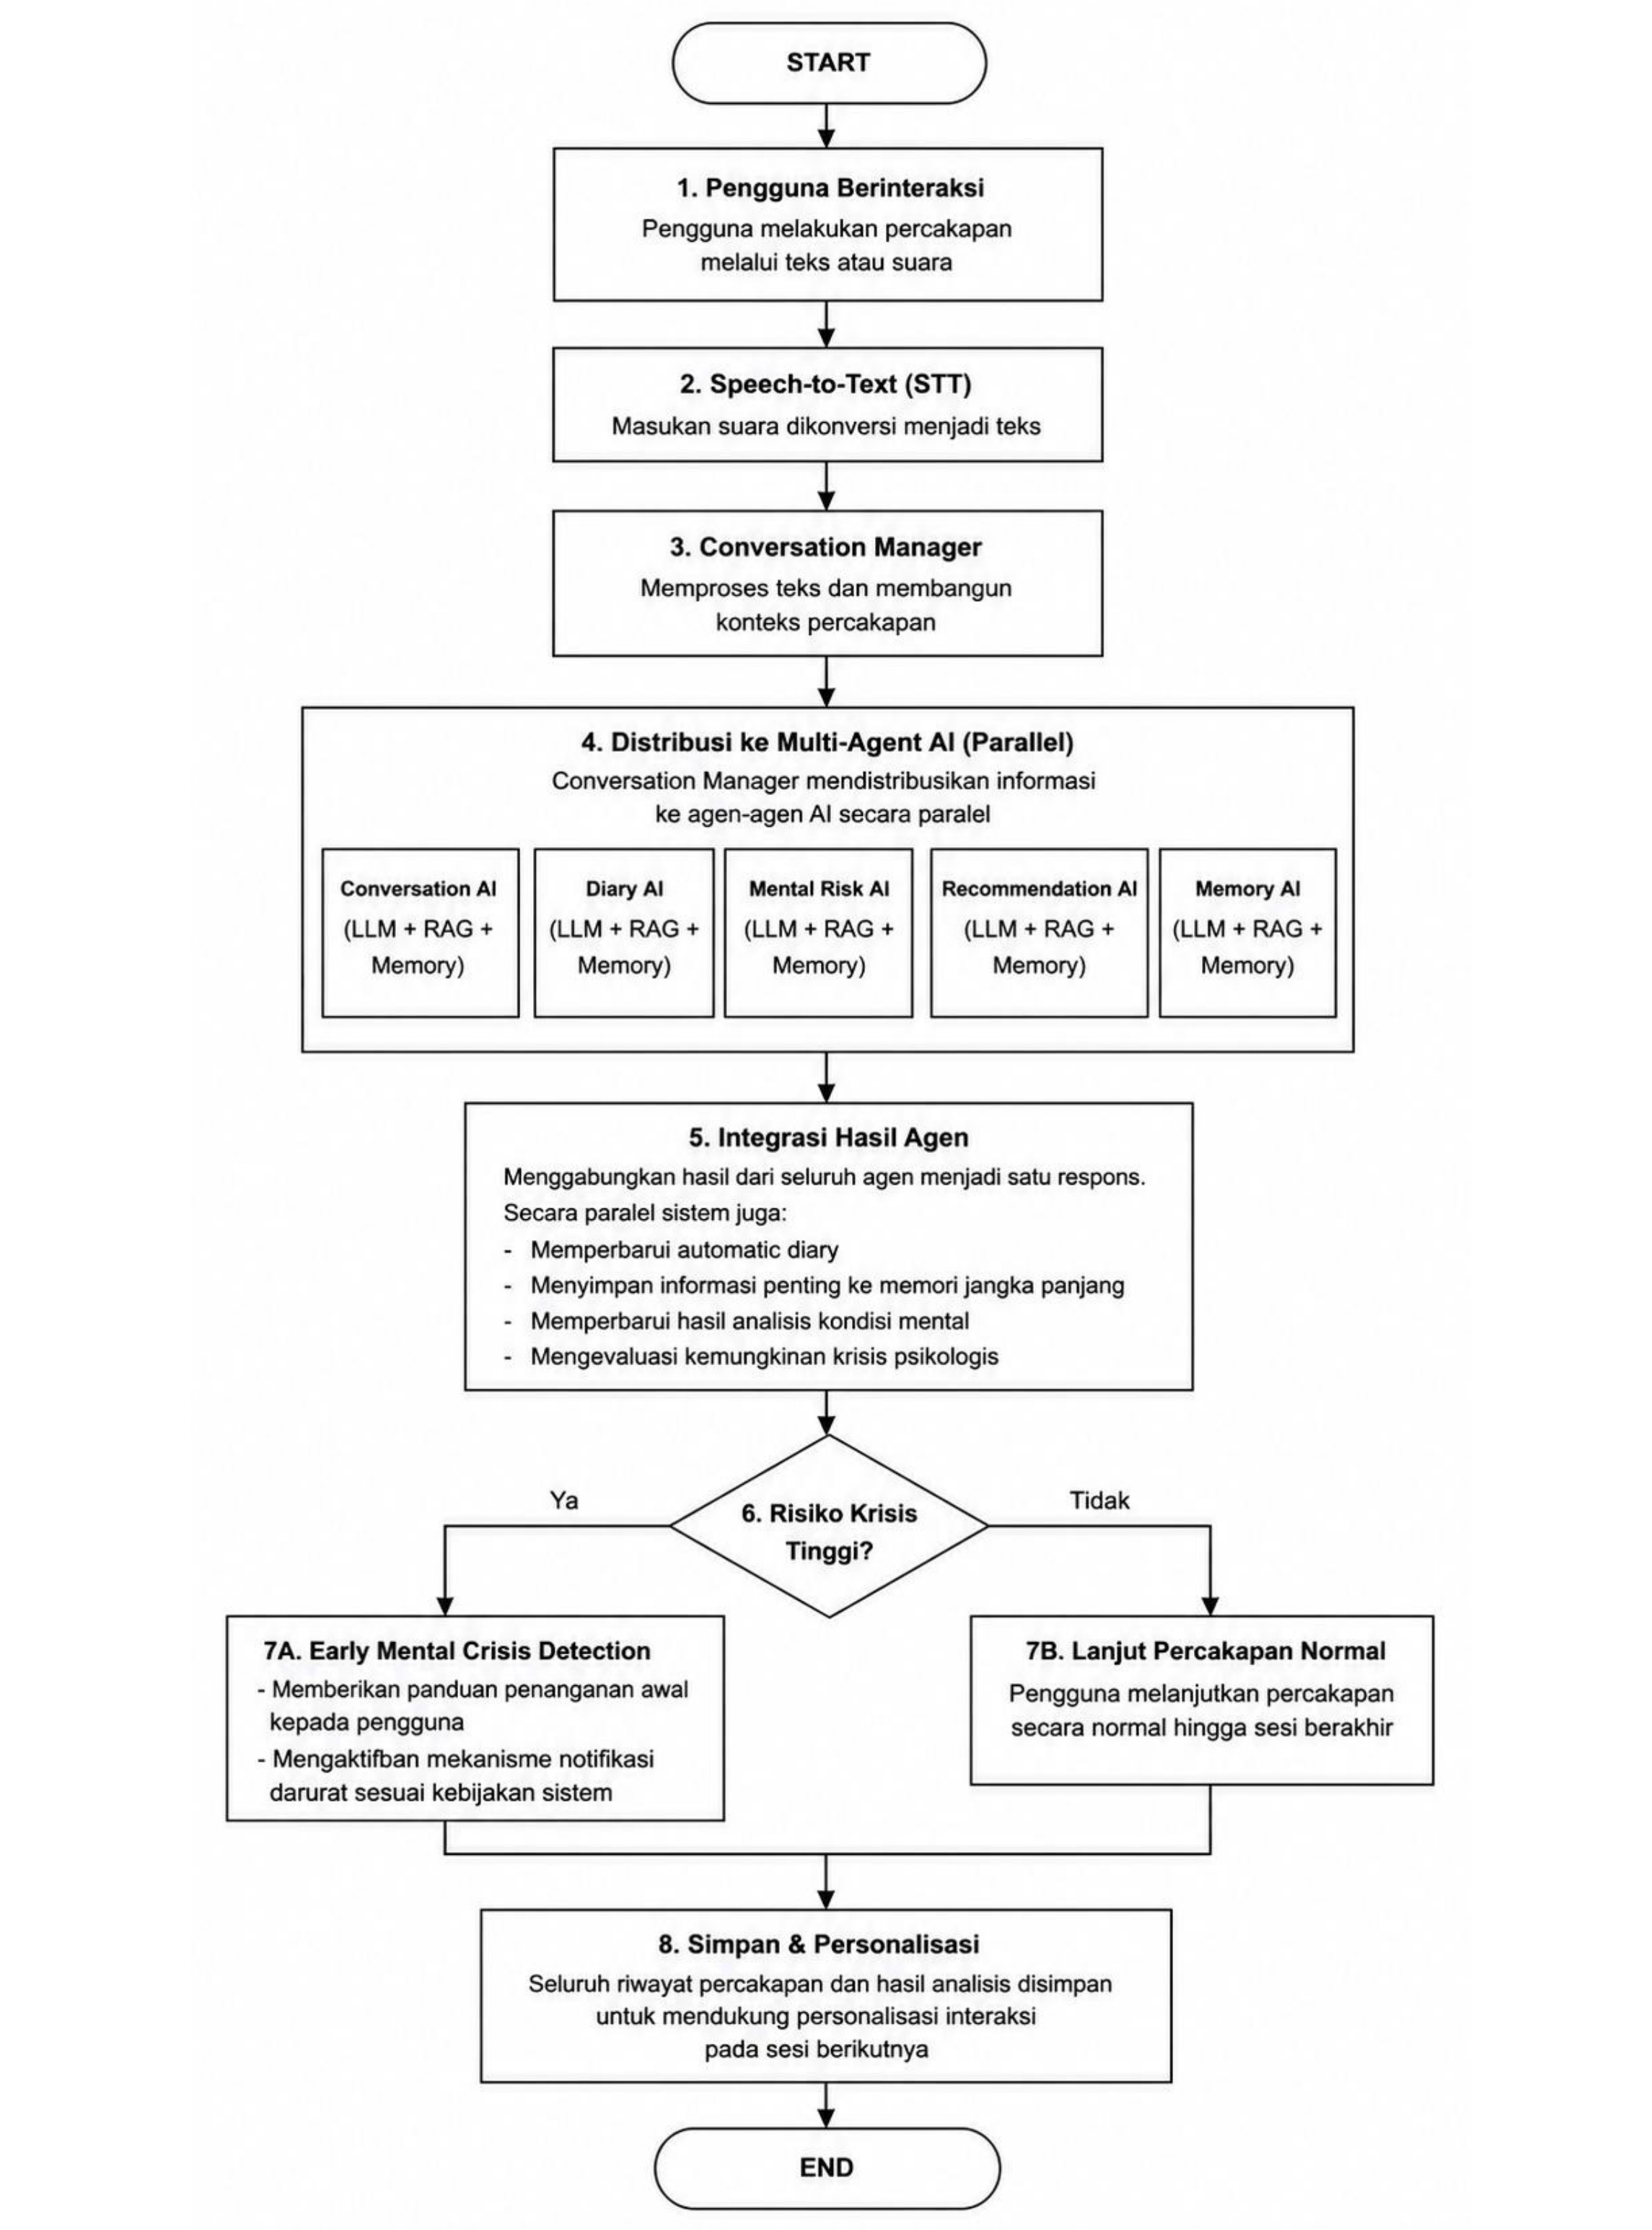
\includegraphics[height=17.5cm,keepaspectratio]{images/bab7/fig5_flow.png}
    \caption{Alur Penggunaan Sistem}
\end{figure}

\subsecbar{7.3 Peran Sistem}
Peran setiap aktor dalam LUNA dirancang untuk mendukung proses pendampingan kesehatan mental secara terintegrasi. Pembagian peran antara pengguna, sistem, komponen Multi-Agent AI, dan layanan notifikasi ditunjukkan pada Tabel 3.

\begin{table}[H]
\centering
\renewcommand{\arraystretch}{1.35}
\renewcommand{\tabularxcolumn}[1]{m{#1}}
\arrayrulecolor{TableBorderColor}
\caption{Peran Sistem}
\vspace{0.3em}
\small
\begin{tabularx}{\textwidth}{| >{\bfseries}l | X |}
\hline
\rowcolor{TableHeaderPurple}
\color{white}\bfseries Aktor & \color{white}\bfseries Peran \\
\hline
Pengguna & Melakukan percakapan melalui teks maupun suara, melihat diary, melihat riwayat, menerima rekomendasi, dan memantau kondisi mental. \\
\hline
\rowcolor{TableAltRowBg}
LUNA & Memberikan pendampingan psikologis awal melalui percakapan yang personal dan adaptif. \\
\hline
Multi-Agent AI & Mengelola percakapan, menyusun diary, menganalisis risiko mental, memberikan rekomendasi, serta mengelola memori percakapan. \\
\hline
\rowcolor{TableAltRowBg}
Notification Center & Mengirimkan notifikasi ketika terdeteksi potensi krisis mental sesuai kebijakan sistem. \\
\hline
\end{tabularx}
\end{table}

% === VIII. Mockup Interface Perangkat Lunak ===
\secbox{VIII.}{Mockup Interface Perangkat Lunak}

Perancangan antarmuka LUNA mengutamakan kemudahan penggunaan (\textit{user-friendly}), kenyamanan interaksi, serta visual yang tenang dan inklusif agar pengguna dapat fokus pada proses pendampingan kesehatan mental. Tangkapan layar antarmuka aplikasi nyata (\textit{real application screenshots}) disusun berdasarkan alur operasional utama dan panduan resmi \textit{Luna AI Rulebook}, meliputi alur pendaftaran, dashboard navigasi, sesi percakapan teks \& panggilan suara \textit{real-time}, tracker suasana hati, sintesis jurnal otomatis, hingga modul intervensi krisis (\textit{Support \& Emergency}). Seluruh rincian antarmuka aplikasi tersebut disajikan pada Lampiran 4.

% === IX. Dokumentasi Cara Penggunaan Perangkat Lunak ===
\secbox{IX.}{Dokumentasi Cara Penggunaan Perangkat Lunak}

Secara umum, penggunaan LUNA dilakukan melalui tahapan berikut:
\begin{enumerate}[leftmargin=*,label=\arabic*.,itemsep=0.15em,parsep=0pt]
    \item Pengguna melakukan masuk (\textit{login}) ke dalam aplikasi.
    \item Pengguna memulai percakapan menggunakan teks atau suara.
    \item Sistem menganalisis percakapan melalui Multi-Agent Artificial Intelligence untuk memahami konteks dan kondisi emosional pengguna.
    \item LUNA memberikan respons pendampingan yang dipersonalisasi sesuai hasil analisis.
    \item Hasil percakapan secara otomatis disusun menjadi diary harian dan disimpan sebagai riwayat pengguna.
    \item Sistem melakukan analisis kondisi mental secara berkelanjutan serta memberikan rekomendasi yang sesuai dengan kebutuhan pengguna.
    \item Apabila terdeteksi indikasi risiko krisis mental, sistem menjalankan mekanisme \textit{Early Mental Crisis Detection} sesuai kebijakan yang diterapkan.
\end{enumerate}

Dokumentasi penggunaan secara rinci setiap langkah disajikan pada Lampiran 5.

\vspace{0.8em}
\subsecbar{1. Rencana Uji Coba Klinis \& Pilot Testing}

\indent Dalam rangka memastikan efektivitas serta keamanan respons pendampingan LUNA pada skenario dunia nyata, tim pengembang telah menginisiasi komunikasi dan kolaborasi awal bersama pakar kesehatan mental, \textbf{Qori Fanani, M.Psi., Psikolog} (Petugas Poliklinik Politeknik Negeri Malang dan Dosen Universitas Kepanjen). Pihak Poliklinik Polinema sangat terbuka untuk mendukung pelaksanaan \textit{clinical pilot testing} dan uji coba penggunaan LUNA kepada mahasiswa maupun pasien di poliklinik. Tahapan rencana uji coba klinis lanjutan yang dirancang meliputi:

\begin{enumerate}[leftmargin=*,label=\arabic*.,itemsep=0.15em,parsep=0pt]
    \item \textbf{Uji Validasi Respons AI oleh Psikolog Klinis:} Evaluasi tingkat empati, kesesuaian modul intervensi CBT, serta presisi kalkulasi skor DASS-21 (Level 1--3) oleh ahli kesehatan mental profesional.
    \item \textbf{Pilot Deployment Terbatas:} Penerapan aplikasi LUNA secara bertahap pada responden pengguna di Poliklinik Polinema di bawah pengawasan psikolog.
    \item \textbf{Evaluasi Dampak \& Refinement:} Pengukuran perubahan skor depresi, kecemasan, dan stres sebelum serta sesudah penggunaan LUNA untuk melakukan penyempurnaan alur agen AI secara berkelanjutan.
\end{enumerate}




% === DAFTAR PUSTAKA ===
\clearpage
\begin{center}
    {\Large\bfseries\color{PrimaryBlue} DAFTAR PUSTAKA\par}
\end{center}
\vspace{1.2em}

\begingroup
\small
\setstretch{1.15}
\setlength{\parindent}{-1.5em}
\setlength{\leftskip}{1.5em}
\setlength{\parskip}{0.6em}

Arrahmi Thahir, F., Adisti Hajarini, F., Nasution, K., Nazira Harahap, T., \& Wulandari, V. (2023). PT. Media Akademik Publisher KESEHATAN MENTAL DI ERA GENERASI Z DALAM STUDI KASUS SMP NEGERI 36 MEDAN. \textit{Jurnal Media Akademik (JMA)}, 1(1), 224--230. \url{https://jurnal.mediaakademik.com/index.php/jma/article/download/18/18}\par

Casey Annie E. (2024). \textit{Masalah Kesehatan Mental Generasi Z}. \url{https://www.aecf.org/blog/generation-z-and-mental-health}\par

Casey Annie E. (2025). \textit{STATISTIK KESEHATAN MENTAL REMAJA}. \url{https://www.aecf.org/blog/youth-mental-health-statistics}\par

Damanik, E. D. (2011). \textit{Pengujian reliabilitas, validitas, analisis butir dan pembuatan norma Depression Anxiety Stress Scale (DASS)}. Tesis Magister, Fakultas Psikologi Universitas Indonesia. \url{https://lib.ui.ac.id/detail.jsp?id=20286884}\par

Dhia Tawakalna, \& Junta Zeniarja. (2026). SISTEM CHATBOT KESEHATAN MENTAL BERBASIS LLM DENGAN DETEKSI EMOSI DAN RETRIEVAL AUGMENTED GENERATION. \textit{Rabit : Jurnal Teknologi Dan Sistem Informasi Univrab}, 11(1), 1398--1412. \url{https://doi.org/10.36341/rabit.v11i1.7347}\par

Elbarbary, K., Alfudoul, A., Samir, A. A., Hussain, H. A. H., Altayib, B., Abdel Al, A. M. A., Jabrieh, G., Shaban, R., Shoib, S., \& El-Gilany, A. H. (2026). Are artificial intelligence chatbots safe for suicide risk assessment? A narratively synthesized review of current evidence. \textit{Cambridge Prisms: Global Mental Health}. \url{https://doi.org/10.1017/gmh.2026.10260}\par

Fadli, R. (2024). \textit{Ini 5 Alasan Gen Z Lebih Rentan Terhadap Gangguan Mental}. Halodoc. \url{https://www.halodoc.com/artikel/ini-5-alasan-gen-z-lebih-rentan-terhadap-gangguan-mental}\par

Fransson, E. (2026). Retrieval-Augmented Generation in Mental Health: A Systematic Review. \textit{Research Gate}. \url{https://doi.org/10.21203/rs.3.rs-10252606/v1}\par

Gong, B., Yao, N., Xie, H., Huang, C., Kishimoto, T., Berenbaum, H., \& Mu, W. (2026). Efficacy, User Engagement, and Acceptability of Cognitive Behavioral Therapy--Oriented Psychological Chatbots for Adults With Depressive and/or Anxiety Symptoms: Systematic Review and Meta-Analysis of Randomized Controlled Trials. \textit{Journal of Medical Internet Research}, 28(1). \url{https://doi.org/10.2196/82677}\par

Lovibond, S. H., \& Lovibond, P. F. (1995). \textit{Manual for the Depression Anxiety Stress Scales} (2nd ed.). Sydney: Psychology Foundation of Australia. \url{https://www2.psy.unsw.edu.au/dass/}\par

Muttaqin, D. (2021). Mengukur depresi, kecemasan, dan stres pada kelompok dewasa awal di Indonesia: Uji validitas dan reliabilitas DASS-21. \textit{Jurnal Psikologi Teori dan Terapan}, 11(2), 153--166. \url{https://doi.org/10.26740/jptt.v11n2.p153-166}\par

Packer, C., Wooders, S., Lin, K., Fang, V., Patil, S. G., Stoica, I., \& Gonzalez, J. E. (2024). MemGPT: Towards LLMs as Operating Systems. \textit{ArXiv}. \url{https://doi.org/10.48550/arXiv.2310.08560}\par

UNICEF. (2025). Studi kesehatan mental menunjukkan Generasi Z kewalahan tetapi tidak gentar menghadapi krisis global yang tiada henti. In \textit{UNICEF}. \url{https://www.unicef.org/partnerships/mental-health-study-shows-gen-zoverwhelmed-undeterred-unrelenting-global-crises}\par

World Health Organization. (2020). \textit{Doing what matters in times of stress: An illustrated guide}. World Health Organization. \url{https://www.who.int/publications/i/item/9789240003927}\par

World Health Organization. (2021a). \textit{Early Adolescent Skills for Emotions (EASE): Group psychological intervention for adolescents with emotional problems}. World Health Organization \& UNICEF. \url{https://www.who.int/publications/i/item/9789240030107}\par

World Health Organization. (2021b). \textit{LIVE LIFE: An implementation guide for suicide prevention in countries}. World Health Organization. \url{https://www.who.int/publications/i/item/9789240026629}\par

\endgroup


% === X. LAMPIRAN ===
\clearpage
\secbox{X.}{LAMPIRAN}

\lampiranhead{1. Business Process / Workflow}
\begin{figure}[H]
    \centering
    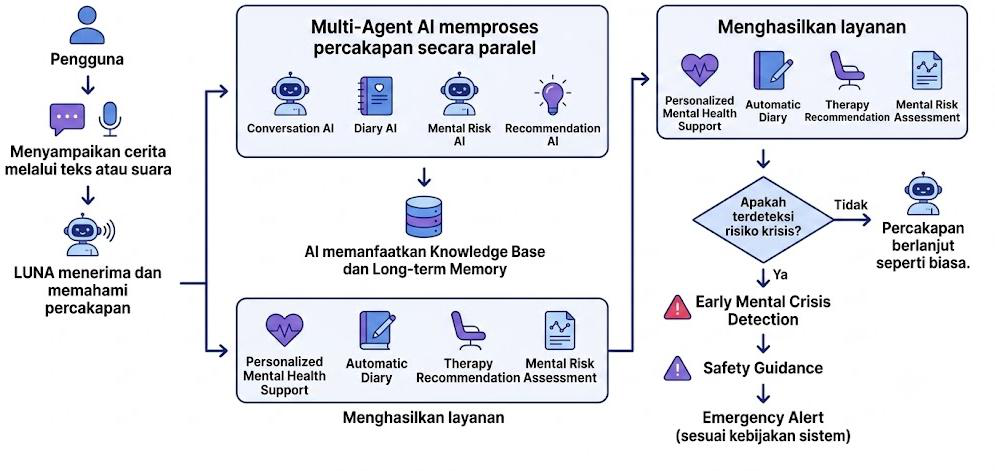
\includegraphics[width=0.92\textwidth]{images/lampiran/fig6_business_process.png}
    \caption{Proses Bisnis LUNA}
\end{figure}

\lampiranhead{2. Use case Diagram}
\begin{figure}[H]
    \centering
    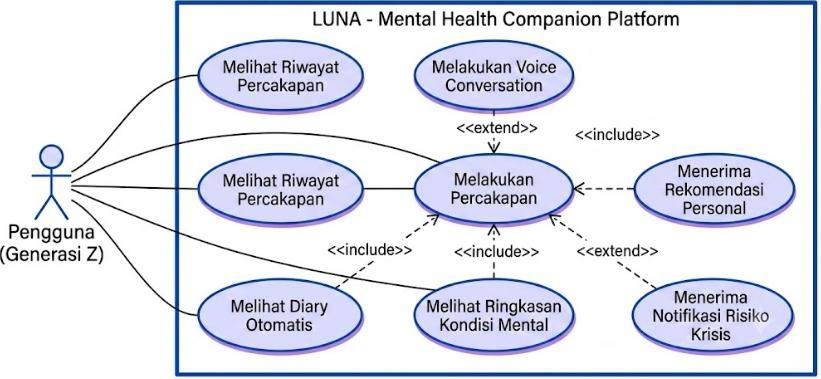
\includegraphics[width=0.88\textwidth]{images/lampiran/fig7_usecase.png}
    \caption{Use Case Diagram}
\end{figure}

\lampiranhead{3. Arsitektur Multi-Agent AI}
\begin{figure}[H]
    \centering
    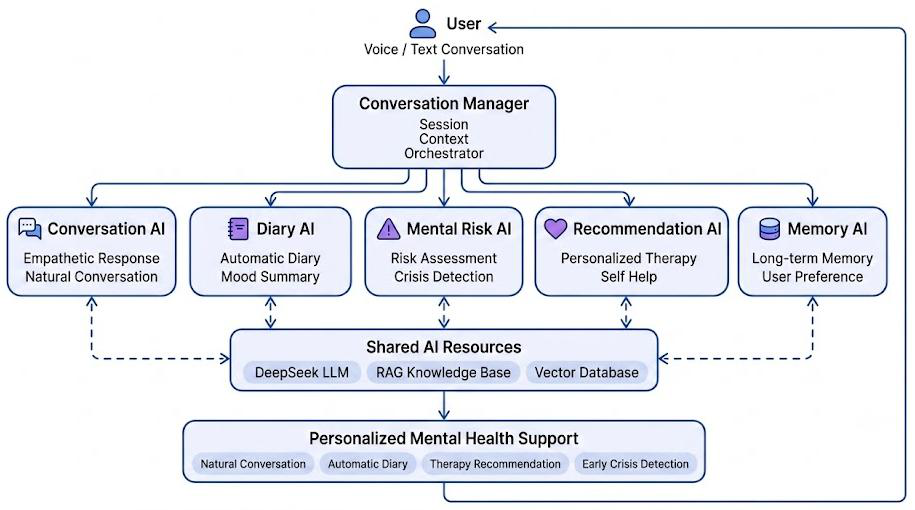
\includegraphics[width=0.92\textwidth]{images/lampiran/fig8_multiagent_architecture.png}
    \caption{Arsitektur Multi-Agent AI}
\end{figure}

\lampiranhead{4. Mockup Interface Application}

\subsubsecstyle{a. Register}
\begin{figure}[H]
    \centering
    \begin{tikzpicture}
        \node[
            draw=TealAccent,
            fill=white,
            line width=0.8pt,
            rounded corners=6pt,
            inner sep=2pt
        ] {
            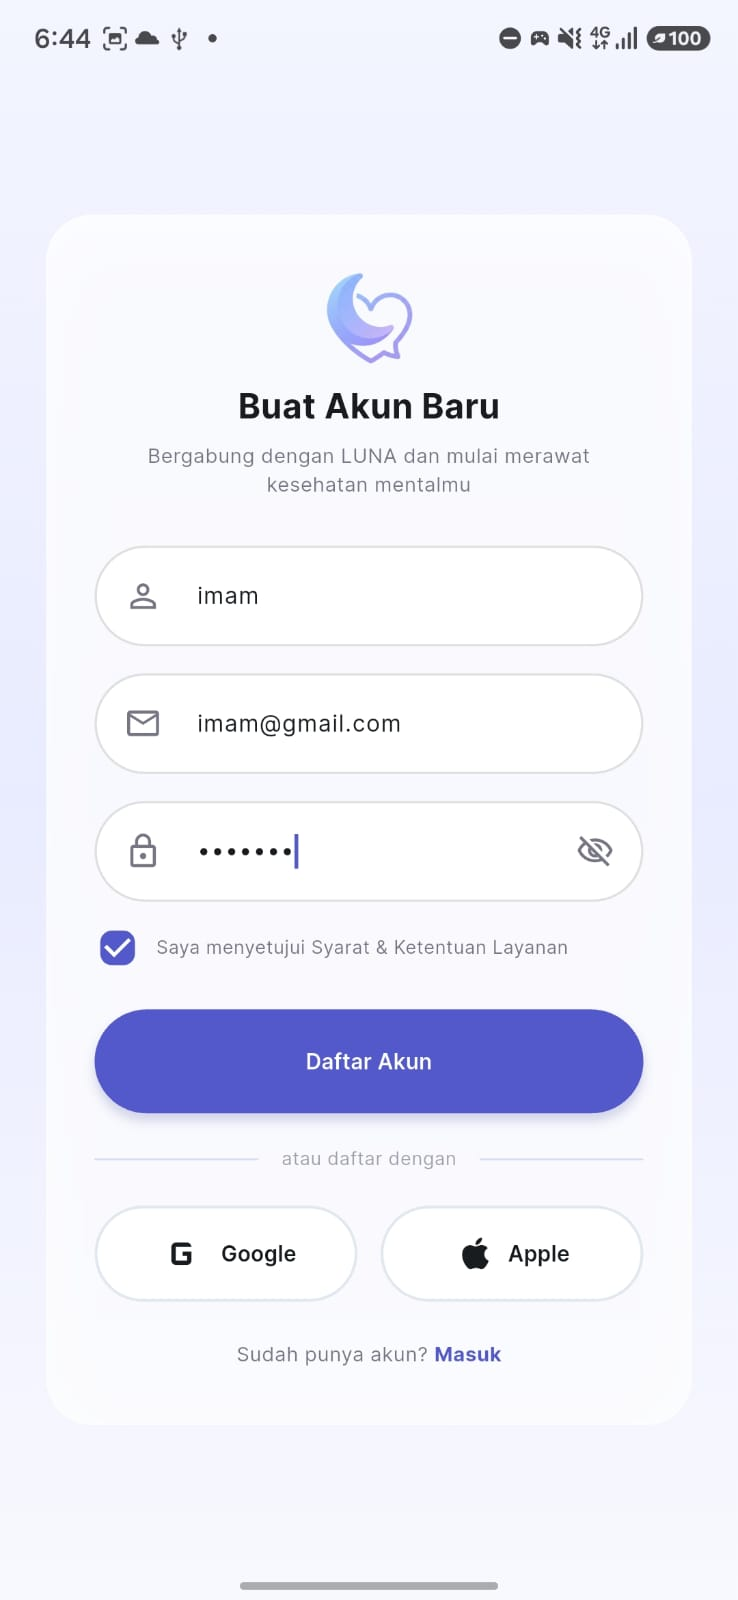
\includegraphics[height=5.8cm,keepaspectratio]{images/prototype/auth_signup.jpeg}
        };
    \end{tikzpicture}
    \caption{Register}
\end{figure}

\subsubsecstyle{b. Login}
\begin{figure}[H]
    \centering
    \begin{tikzpicture}
        \node[
            draw=TealAccent,
            fill=white,
            line width=0.8pt,
            rounded corners=6pt,
            inner sep=2pt
        ] {
            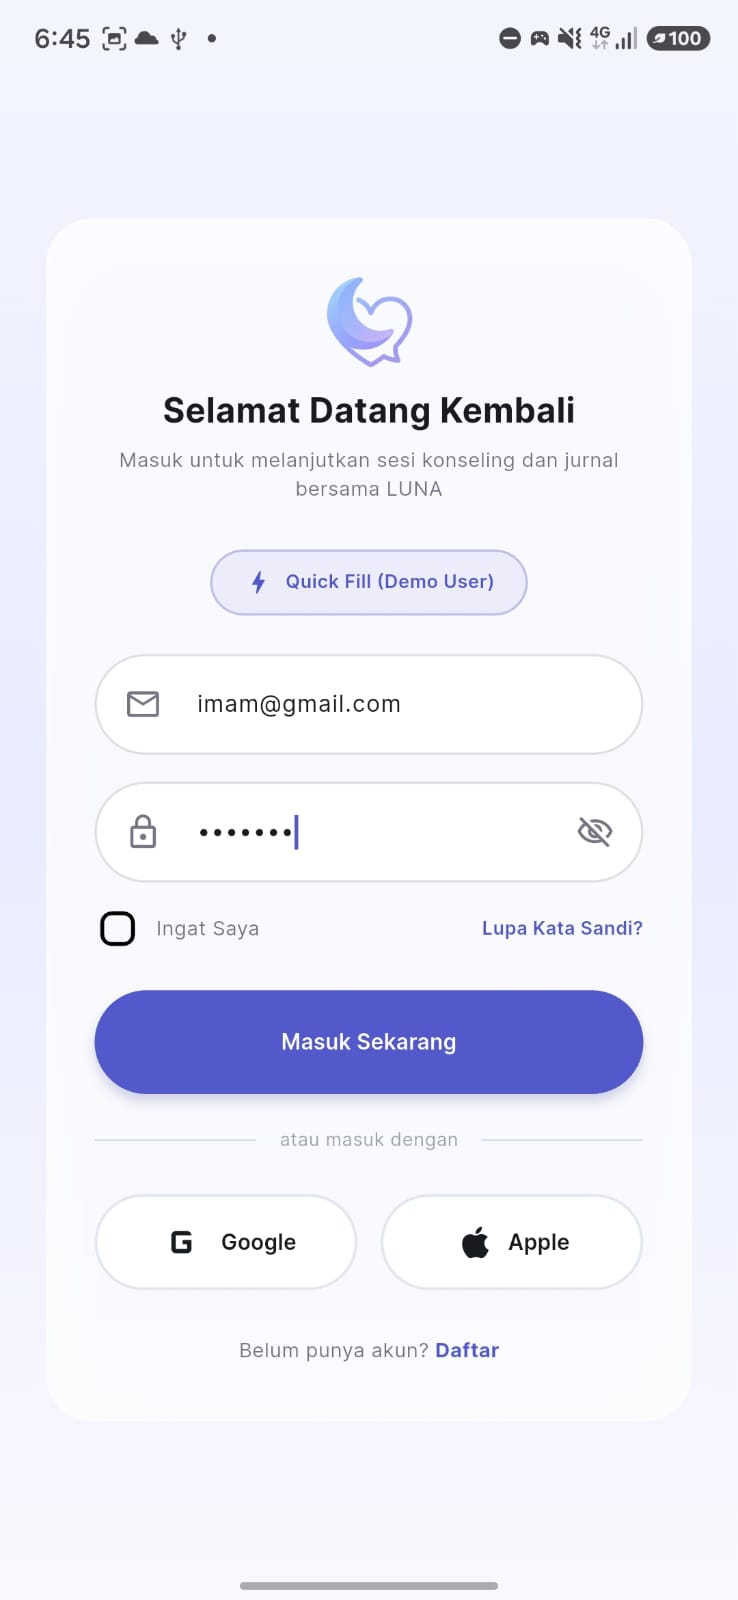
\includegraphics[height=5.8cm,keepaspectratio]{images/prototype/auth_signin.jpeg}
        };
    \end{tikzpicture}
    \caption{Login}
\end{figure}

\subsubsecstyle{c. Onboarding}
\begin{figure}[H]
    \centering
    \begin{tikzpicture}
        \node[
            draw=TealAccent,
            fill=white,
            line width=0.8pt,
            rounded corners=6pt,
            inner sep=2pt
        ] {
            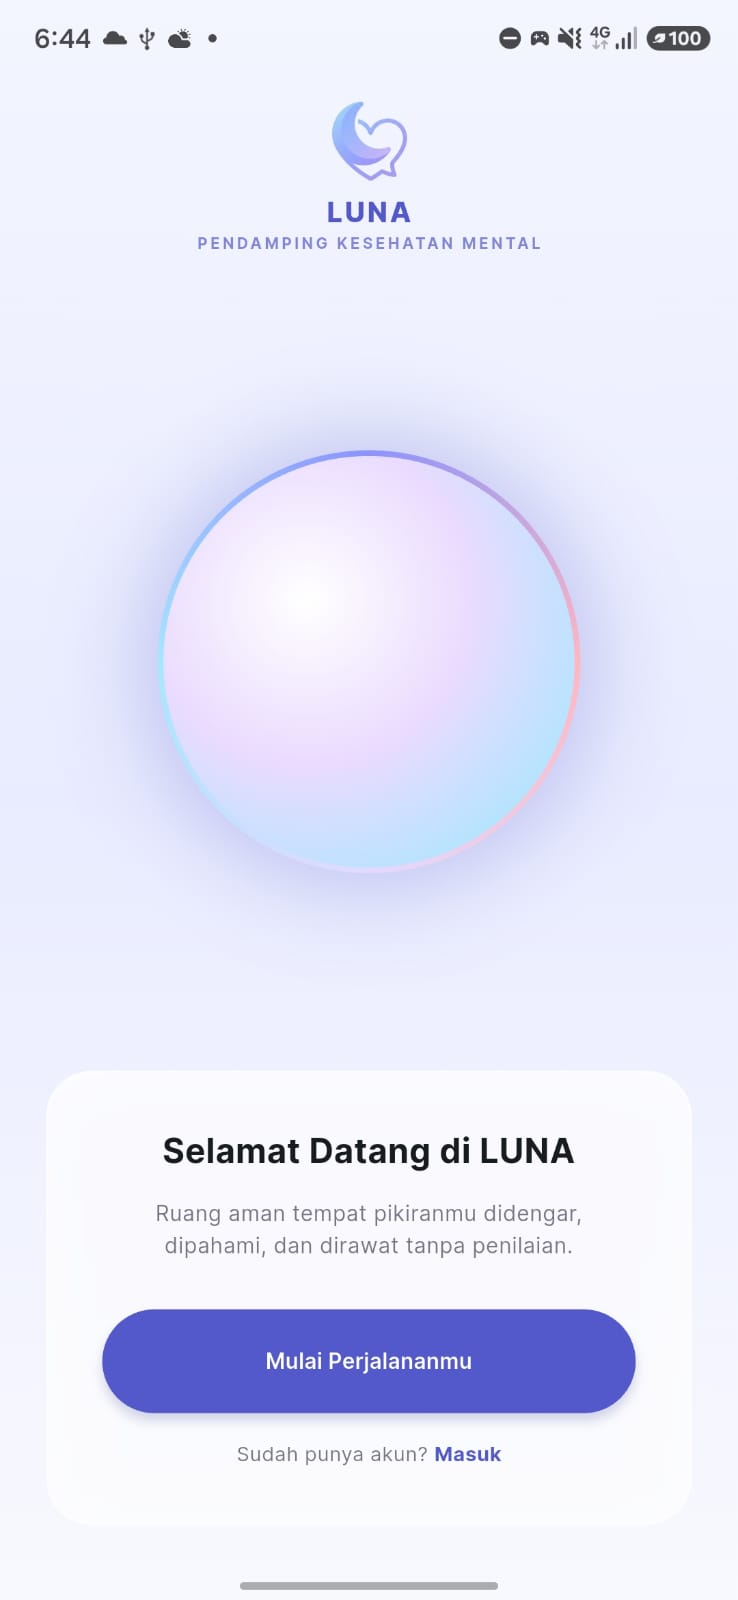
\includegraphics[height=5.8cm,keepaspectratio]{images/prototype/auth_firstscreen.jpeg}
        };
    \end{tikzpicture}
    \caption{Onboarding}
\end{figure}

\subsubsecstyle{d. Home}
\begin{figure}[H]
    \centering
    \begin{tikzpicture}
        \node[
            draw=TealAccent,
            fill=white,
            line width=0.8pt,
            rounded corners=6pt,
            inner sep=2pt
        ] {
            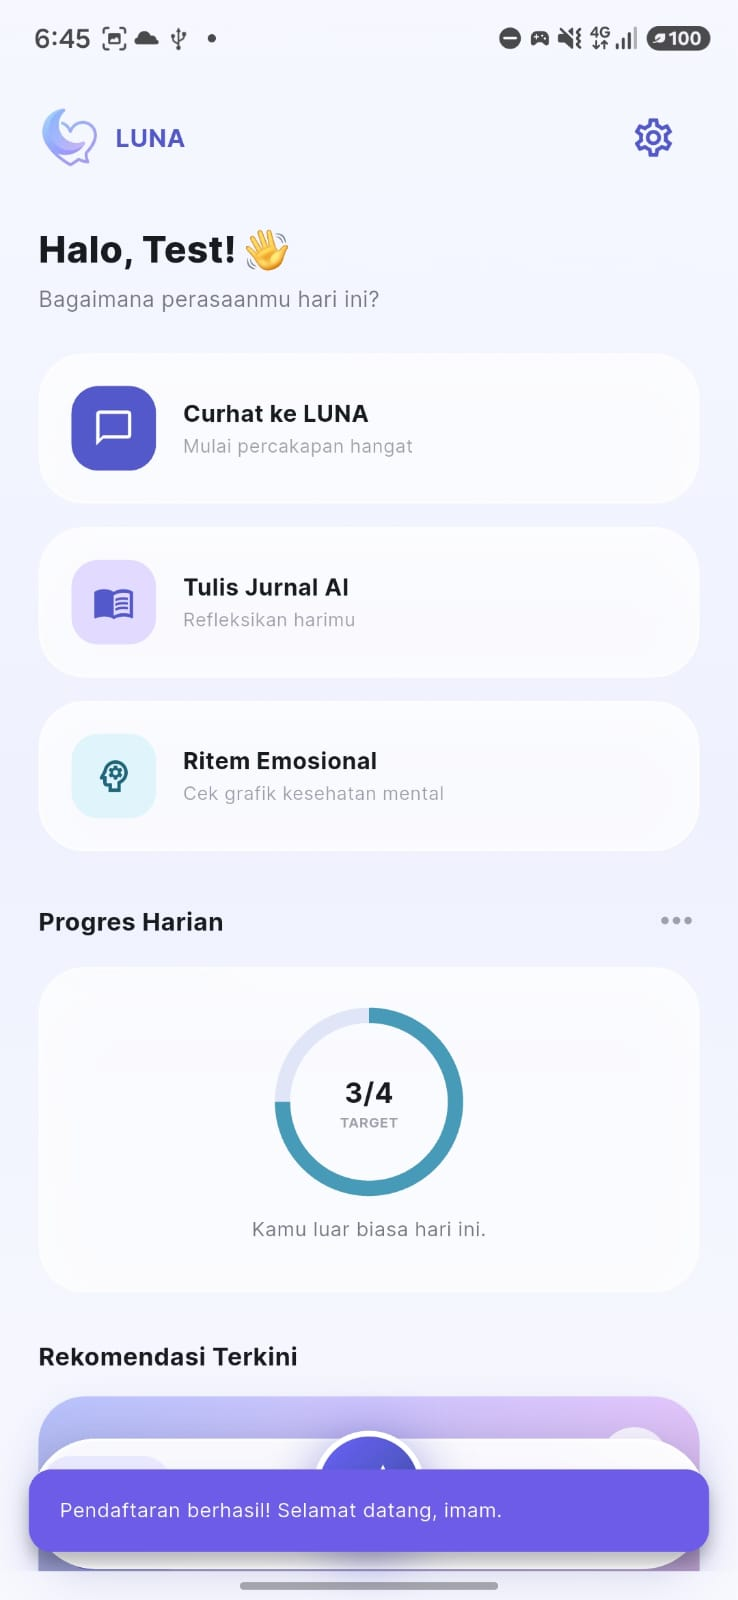
\includegraphics[height=5.8cm,keepaspectratio]{images/prototype/auth_home.jpeg}
        };
    \end{tikzpicture}
    \caption{Home}
\end{figure}

\subsubsecstyle{e. AI Conversation}
\begin{figure}[H]
    \centering
    \begin{minipage}[b]{0.45\textwidth}
        \centering
        \begin{tikzpicture}
            \node[
                draw=TealAccent,
                fill=white,
                line width=0.8pt,
                rounded corners=6pt,
                inner sep=2pt
            ] {
                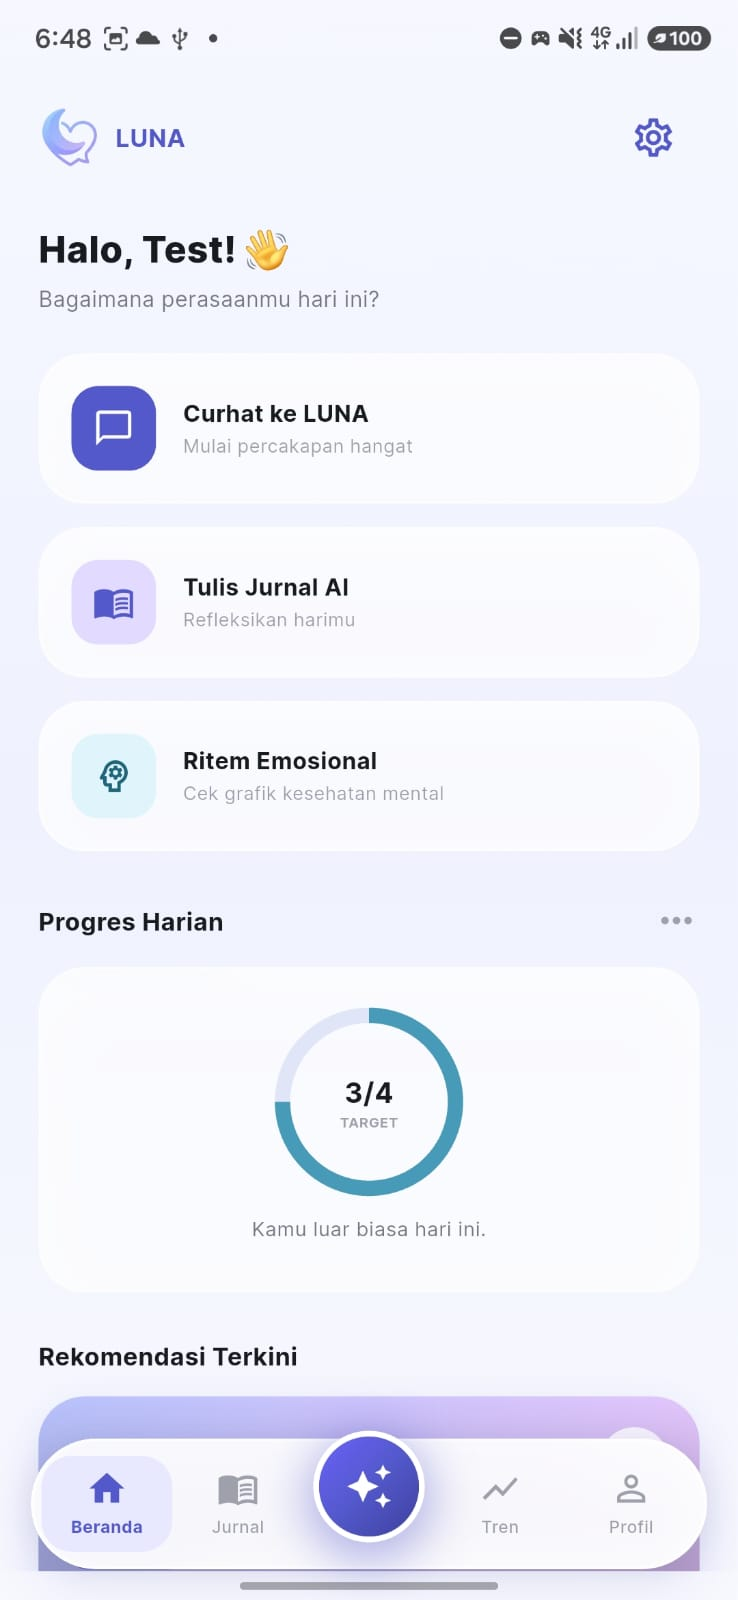
\includegraphics[height=5.8cm,keepaspectratio]{images/prototype/counseling_nav.jpeg}
            };
        \end{tikzpicture}\\[0.3em]
        {\small\itshape (a) Antarmuka Percakapan Teks}
    \end{minipage}%
    \hfill
    \begin{minipage}[b]{0.45\textwidth}
        \centering
        \begin{tikzpicture}
            \node[
                draw=TealAccent,
                fill=white,
                line width=0.8pt,
                rounded corners=6pt,
                inner sep=2pt
            ] {
                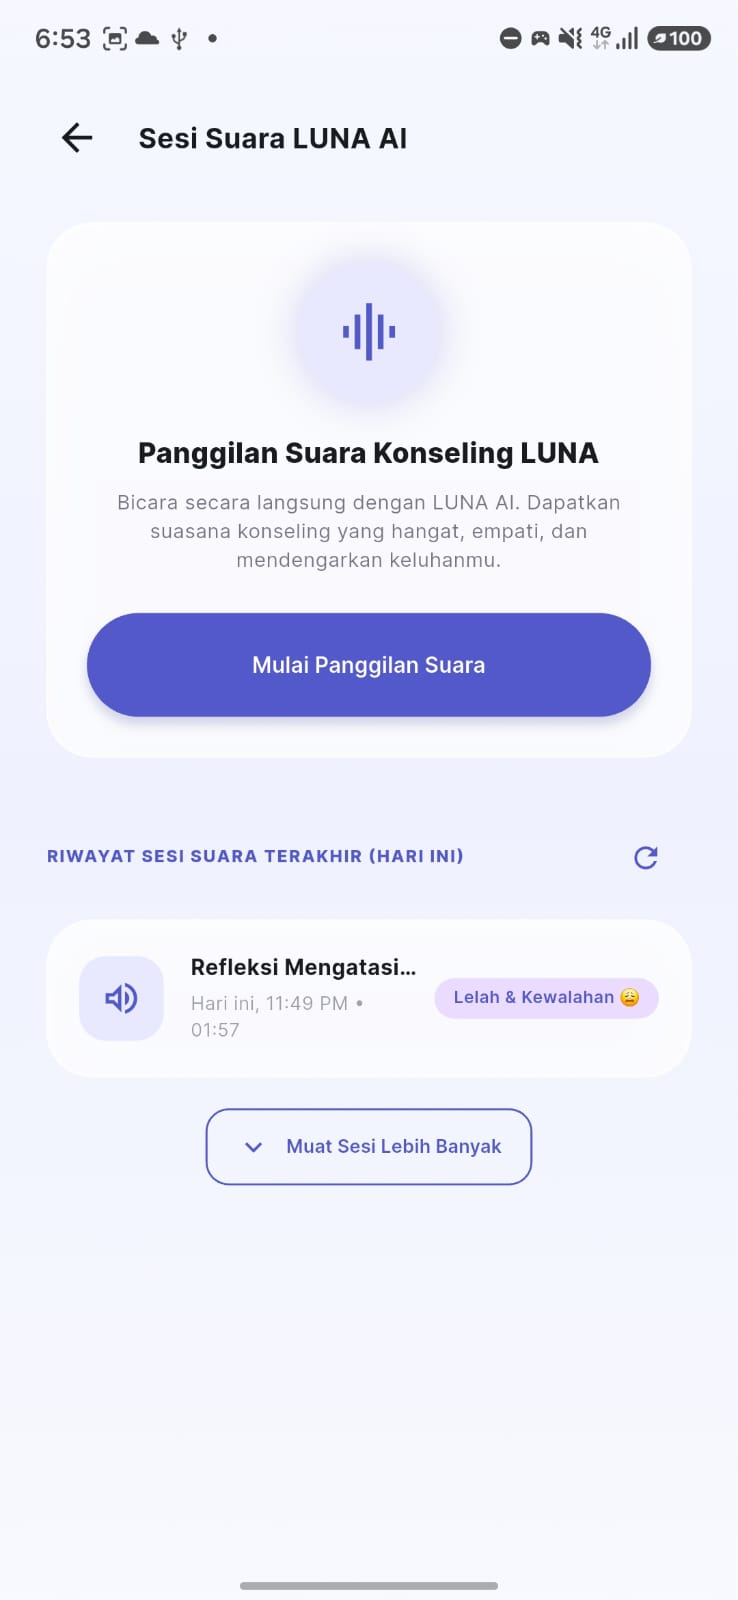
\includegraphics[height=5.8cm,keepaspectratio]{images/prototype/counseling_voice_entry.jpeg}
            };
        \end{tikzpicture}\\[0.3em]
        {\small\itshape (b) Penyiapan Sesi Suara}
    \end{minipage}
    \vspace{0.2em}
    \caption{AI Conversation}
\end{figure}

\subsubsecstyle{f. Voice Call}
\begin{figure}[H]
    \centering
    \begin{minipage}[b]{0.45\textwidth}
        \centering
        \begin{tikzpicture}
            \node[
                draw=TealAccent,
                fill=white,
                line width=0.8pt,
                rounded corners=6pt,
                inner sep=2pt
            ] {
                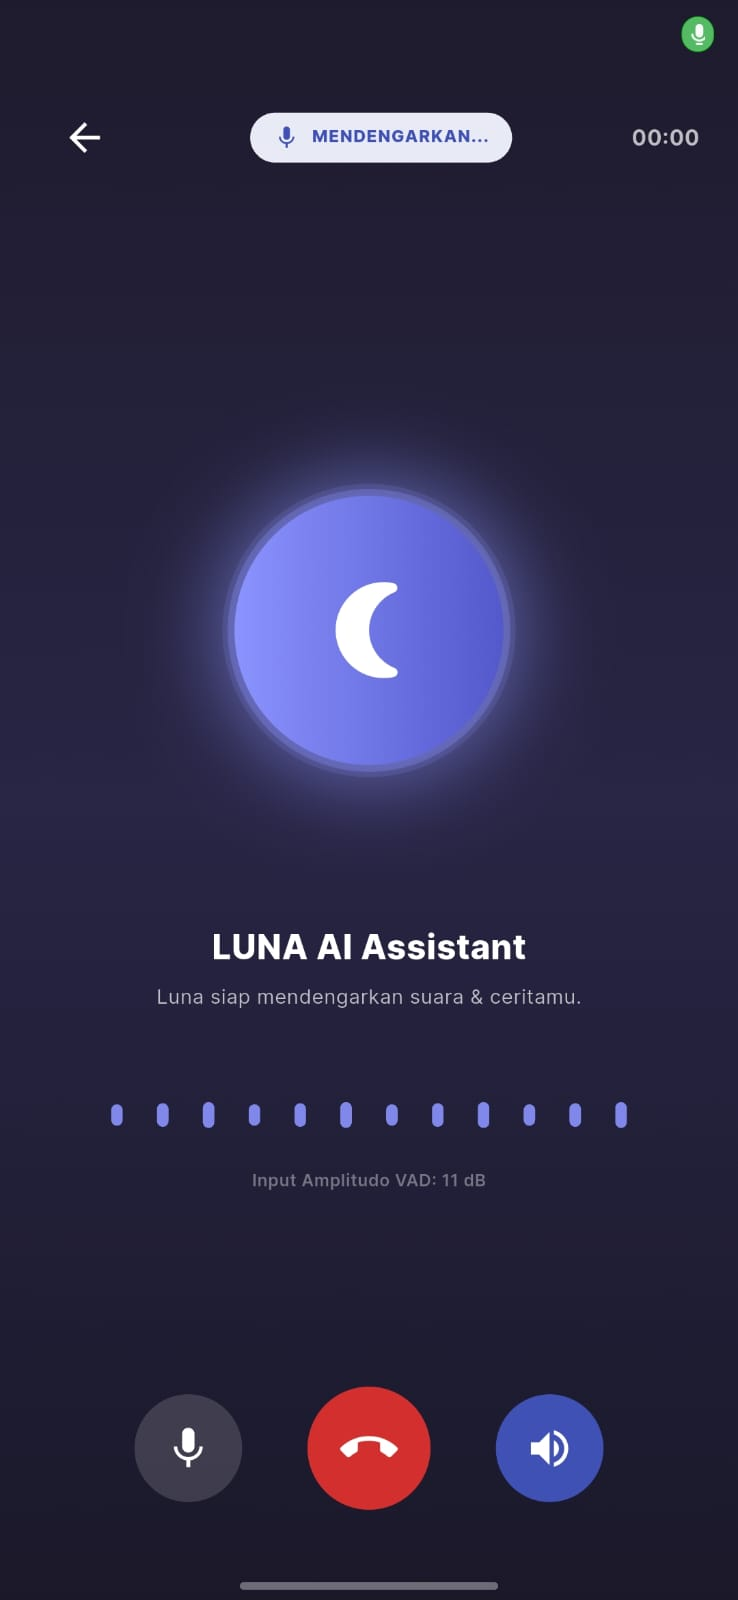
\includegraphics[height=5.8cm,keepaspectratio]{images/prototype/counseling_in_call.jpeg}
            };
        \end{tikzpicture}\\[0.3em]
        {\small\itshape (a) Panggilan Suara Real-Time Aktif}
    \end{minipage}%
    \hfill
    \begin{minipage}[b]{0.45\textwidth}
        \centering
        \begin{tikzpicture}
            \node[
                draw=TealAccent,
                fill=white,
                line width=0.8pt,
                rounded corners=6pt,
                inner sep=2pt
            ] {
                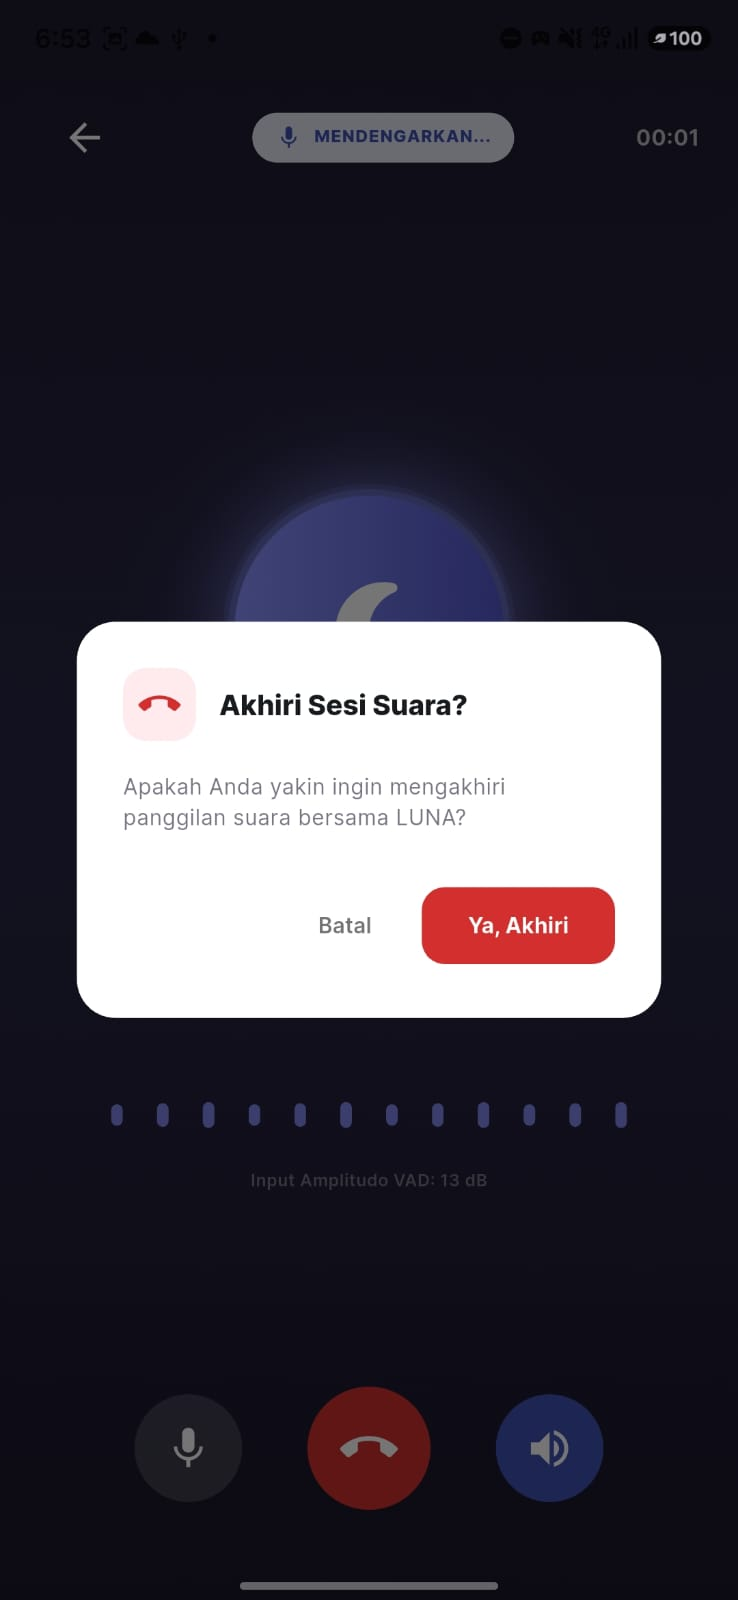
\includegraphics[height=5.8cm,keepaspectratio]{images/prototype/counseling_end_call.jpeg}
            };
        \end{tikzpicture}\\[0.3em]
        {\small\itshape (b) Kontrol \& Penghentian Panggilan}
    \end{minipage}
    \vspace{0.2em}
    \caption{Voice Call}
\end{figure}

\subsubsecstyle{g. AI Diary}
\begin{figure}[H]
    \centering
    \begin{minipage}[b]{0.45\textwidth}
        \centering
        \begin{tikzpicture}
            \node[
                draw=TealAccent,
                fill=white,
                line width=0.8pt,
                rounded corners=6pt,
                inner sep=2pt
            ] {
                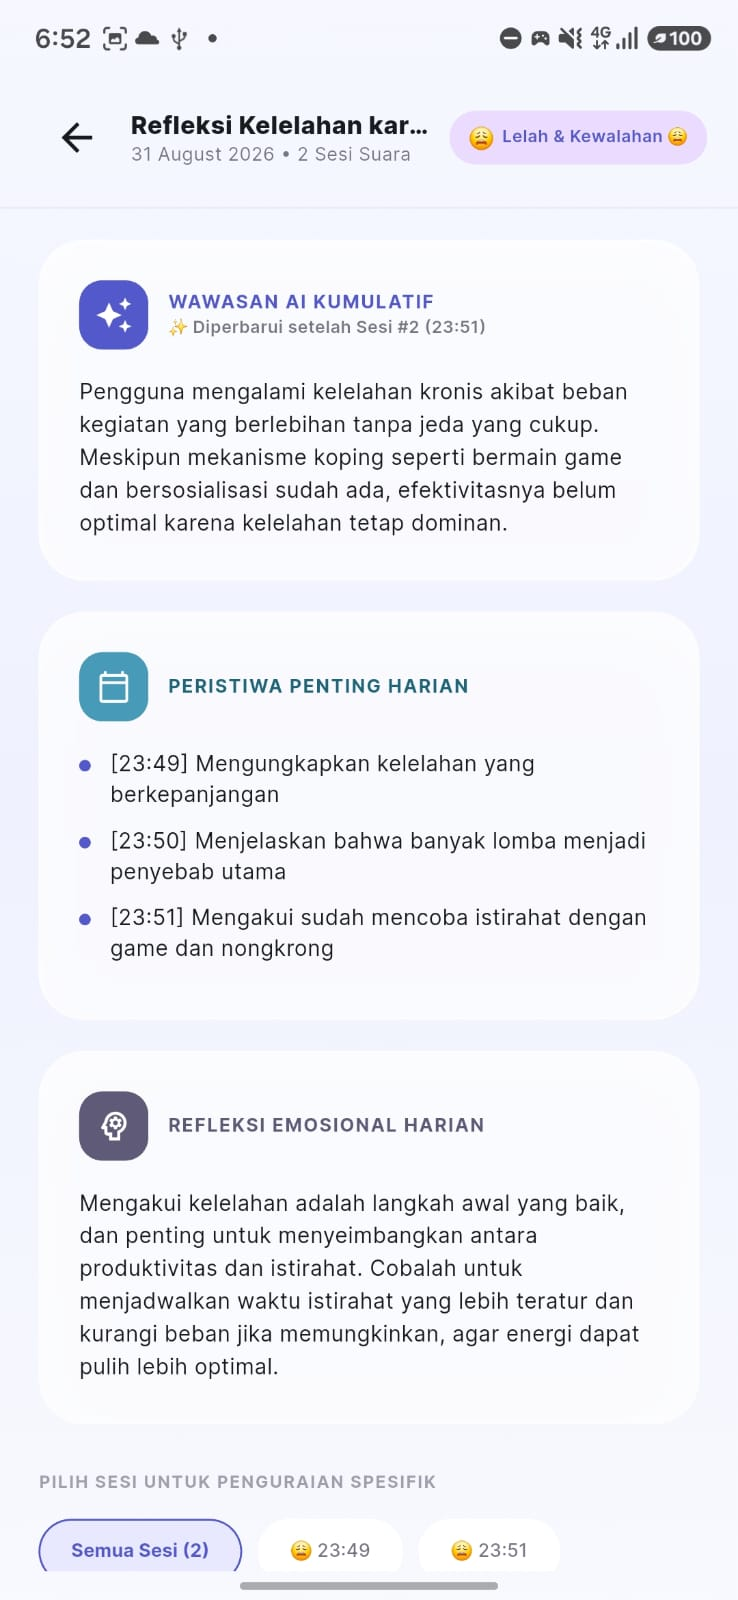
\includegraphics[height=5.8cm,keepaspectratio]{images/prototype/journal_page_1.jpeg}
            };
        \end{tikzpicture}\\[0.3em]
        {\small\itshape (a) Daftar Sintesis Jurnal Harian}
    \end{minipage}%
    \hfill
    \begin{minipage}[b]{0.45\textwidth}
        \centering
        \begin{tikzpicture}
            \node[
                draw=TealAccent,
                fill=white,
                line width=0.8pt,
                rounded corners=6pt,
                inner sep=2pt
            ] {
                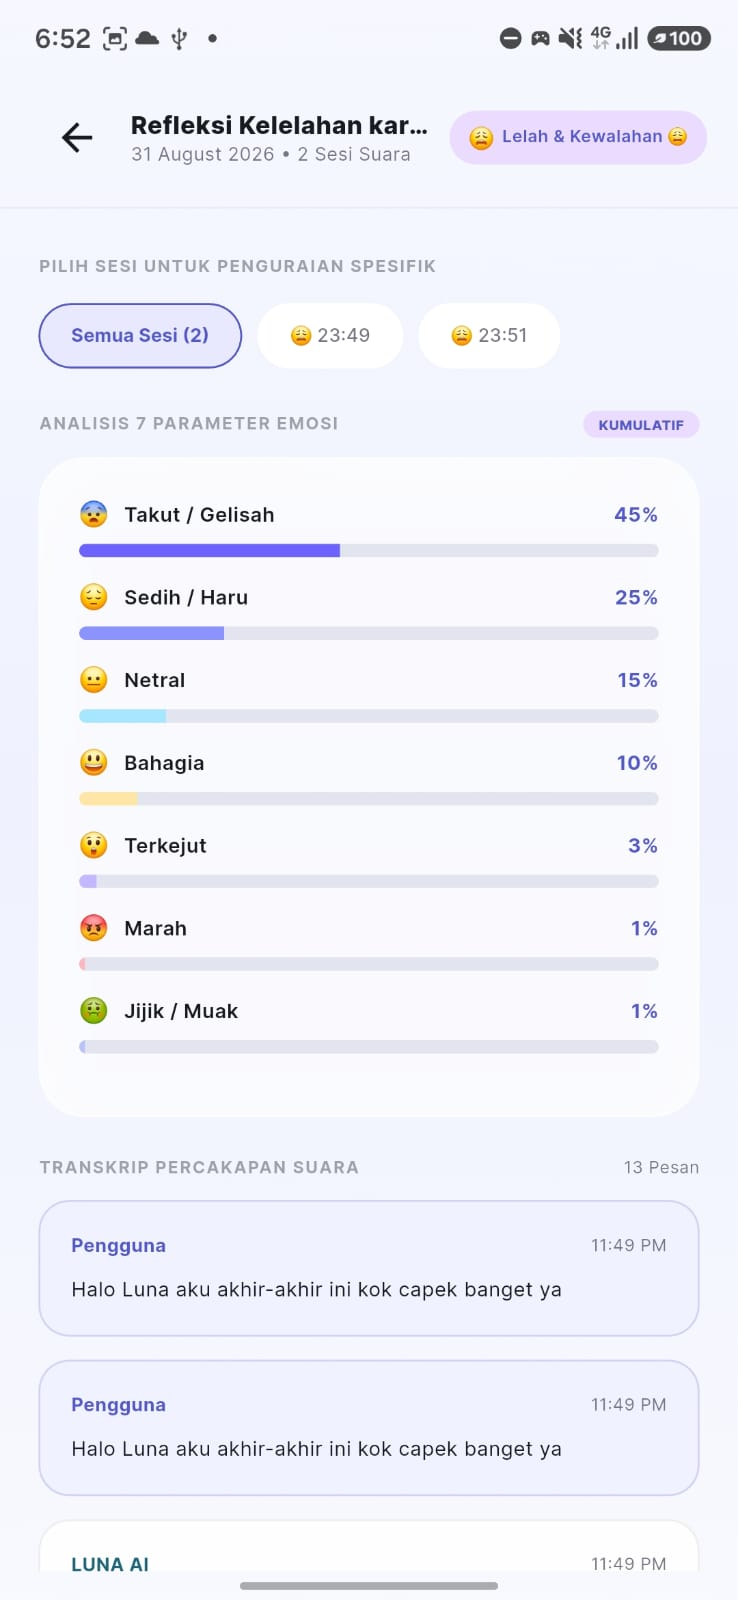
\includegraphics[height=5.8cm,keepaspectratio]{images/prototype/journal_page_2.jpeg}
            };
        \end{tikzpicture}\\[0.3em]
        {\small\itshape (b) Detail Analisis Jurnal Emosional}
    \end{minipage}
    \vspace{0.2em}
    \caption{AI Diary}
\end{figure}

\subsubsecstyle{h. Mental Health Monitoring}
\begin{figure}[H]
    \centering
    \begin{minipage}[b]{0.45\textwidth}
        \centering
        \begin{tikzpicture}
            \node[
                draw=TealAccent,
                fill=white,
                line width=0.8pt,
                rounded corners=6pt,
                inner sep=2pt
            ] {
                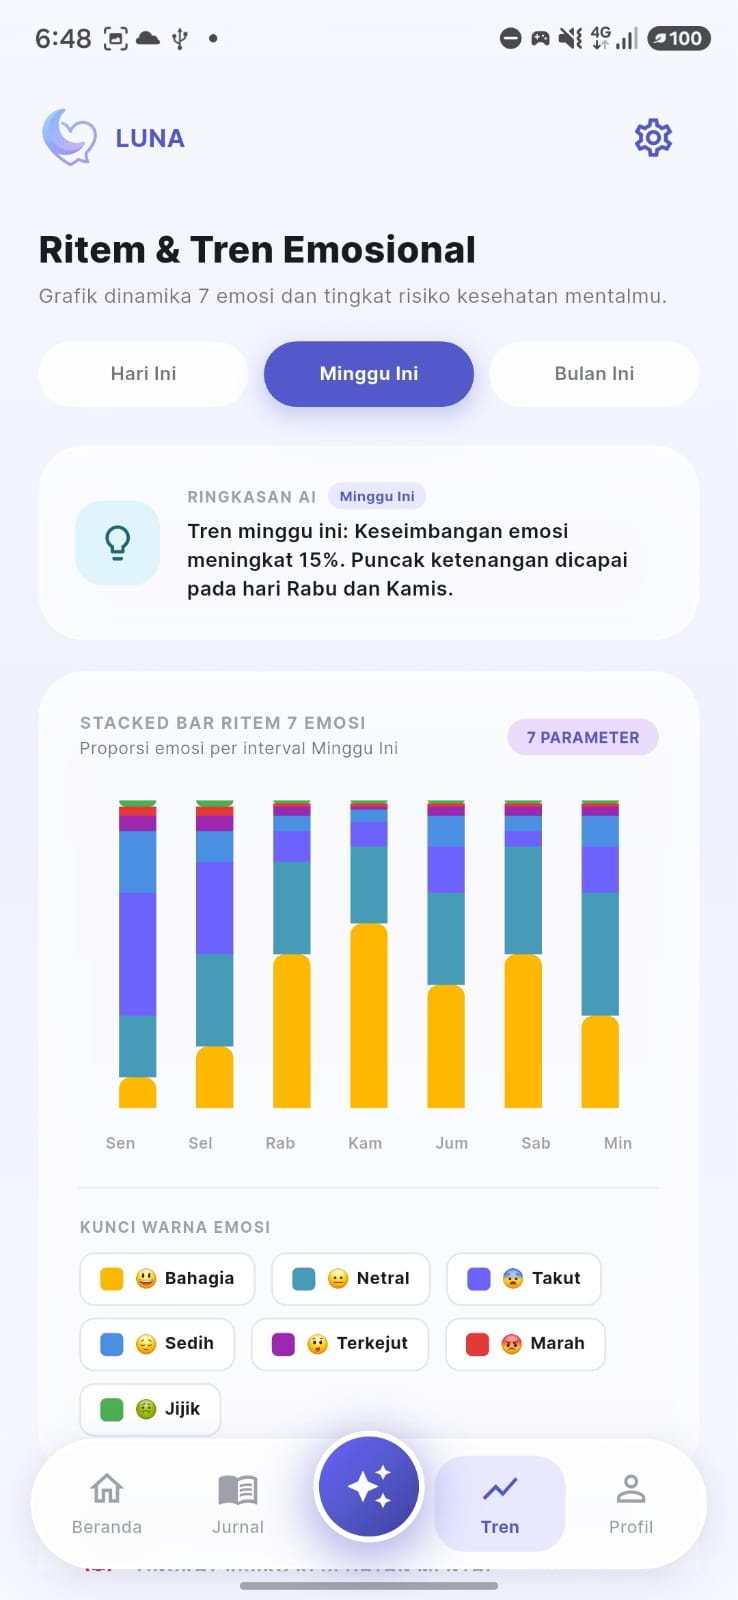
\includegraphics[height=5.8cm,keepaspectratio]{images/prototype/dashboard_page_1.jpeg}
            };
        \end{tikzpicture}\\[0.3em]
        {\small\itshape (a) Mood Tracker Harian}
    \end{minipage}%
    \hfill
    \begin{minipage}[b]{0.45\textwidth}
        \centering
        \begin{tikzpicture}
            \node[
                draw=TealAccent,
                fill=white,
                line width=0.8pt,
                rounded corners=6pt,
                inner sep=2pt
            ] {
                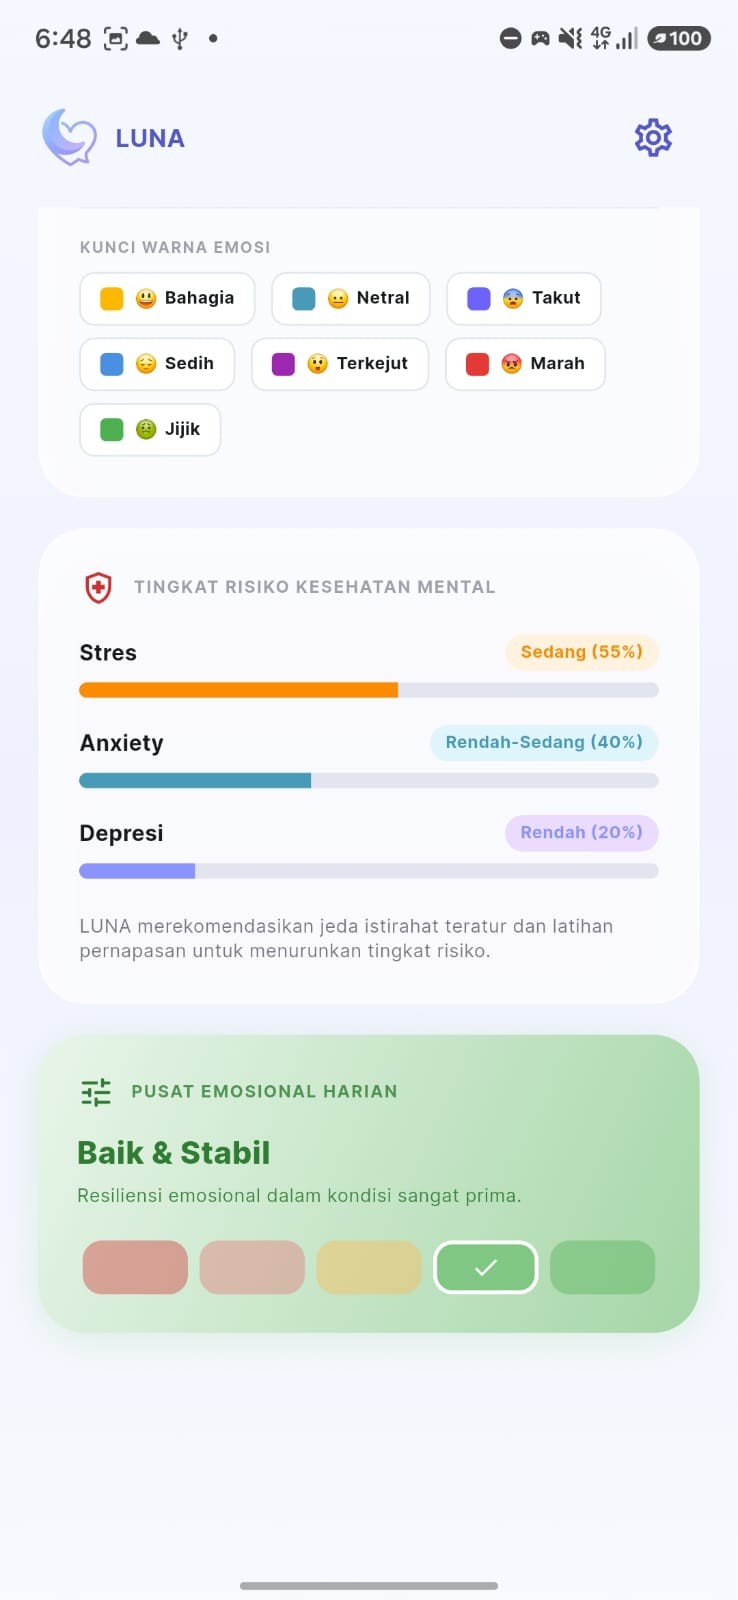
\includegraphics[height=5.8cm,keepaspectratio]{images/prototype/dashboard_page_2.jpeg}
            };
        \end{tikzpicture}\\[0.3em]
        {\small\itshape (b) Grafik Analisis Tren Emosional}
    \end{minipage}
    \vspace{0.2em}
    \caption{Mental Health Monitoring}
\end{figure}

\subsubsecstyle{i. Personalized Recommendation}
\begin{figure}[H]
    \centering
    \begin{minipage}[b]{0.45\textwidth}
        \centering
        \begin{tikzpicture}
            \node[
                draw=TealAccent,
                fill=white,
                line width=0.8pt,
                rounded corners=6pt,
                inner sep=2pt
            ] {
                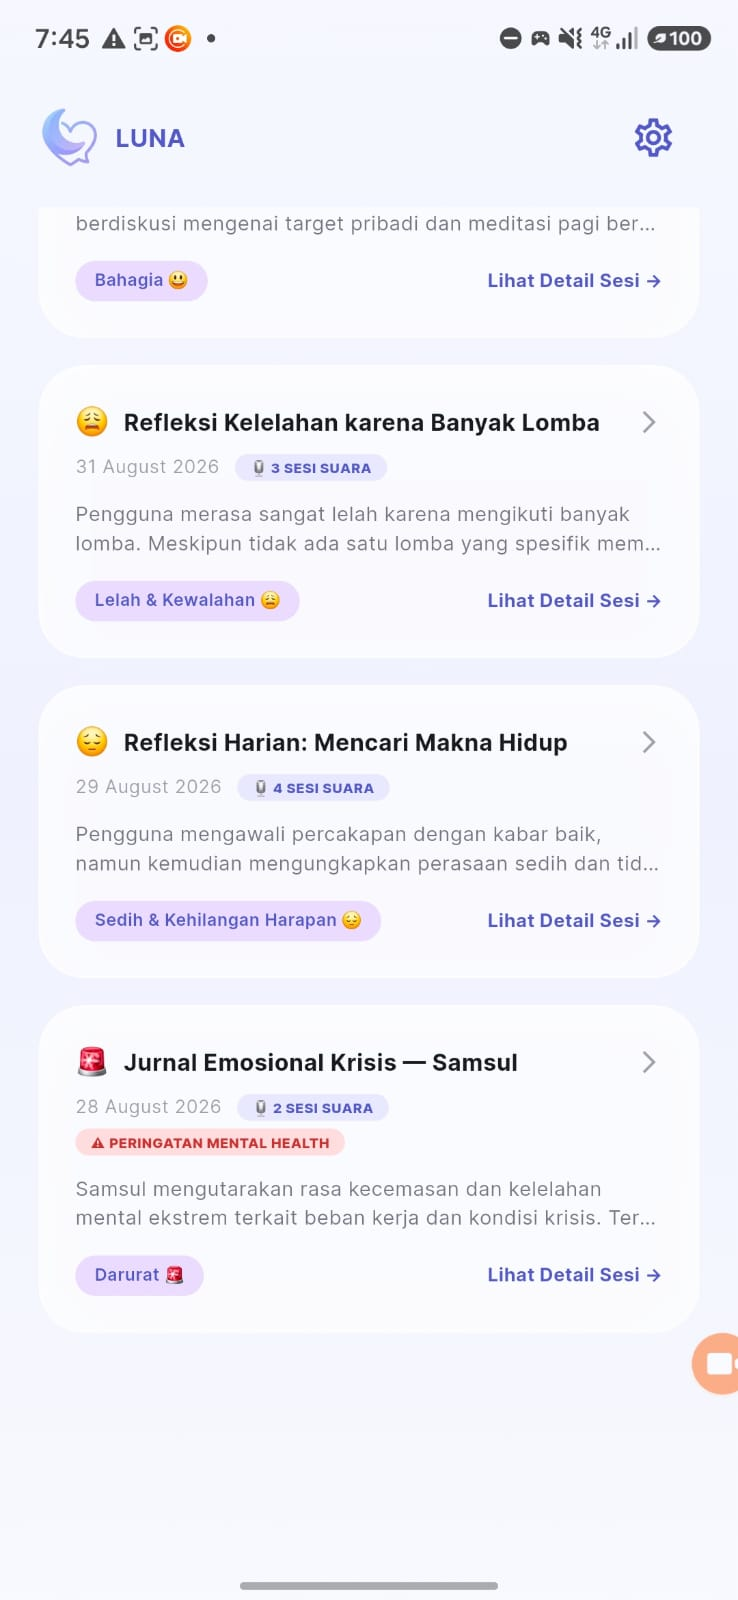
\includegraphics[height=5.8cm,keepaspectratio]{images/prototype/journal_list_crisis.jpeg}
            };
        \end{tikzpicture}\\[0.3em]
        {\small\itshape (a) Daftar Jurnal Risiko Tinggi}
    \end{minipage}%
    \hfill
    \begin{minipage}[b]{0.45\textwidth}
        \centering
        \begin{tikzpicture}
            \node[
                draw=TealAccent,
                fill=white,
                line width=0.8pt,
                rounded corners=6pt,
                inner sep=2pt
            ] {
                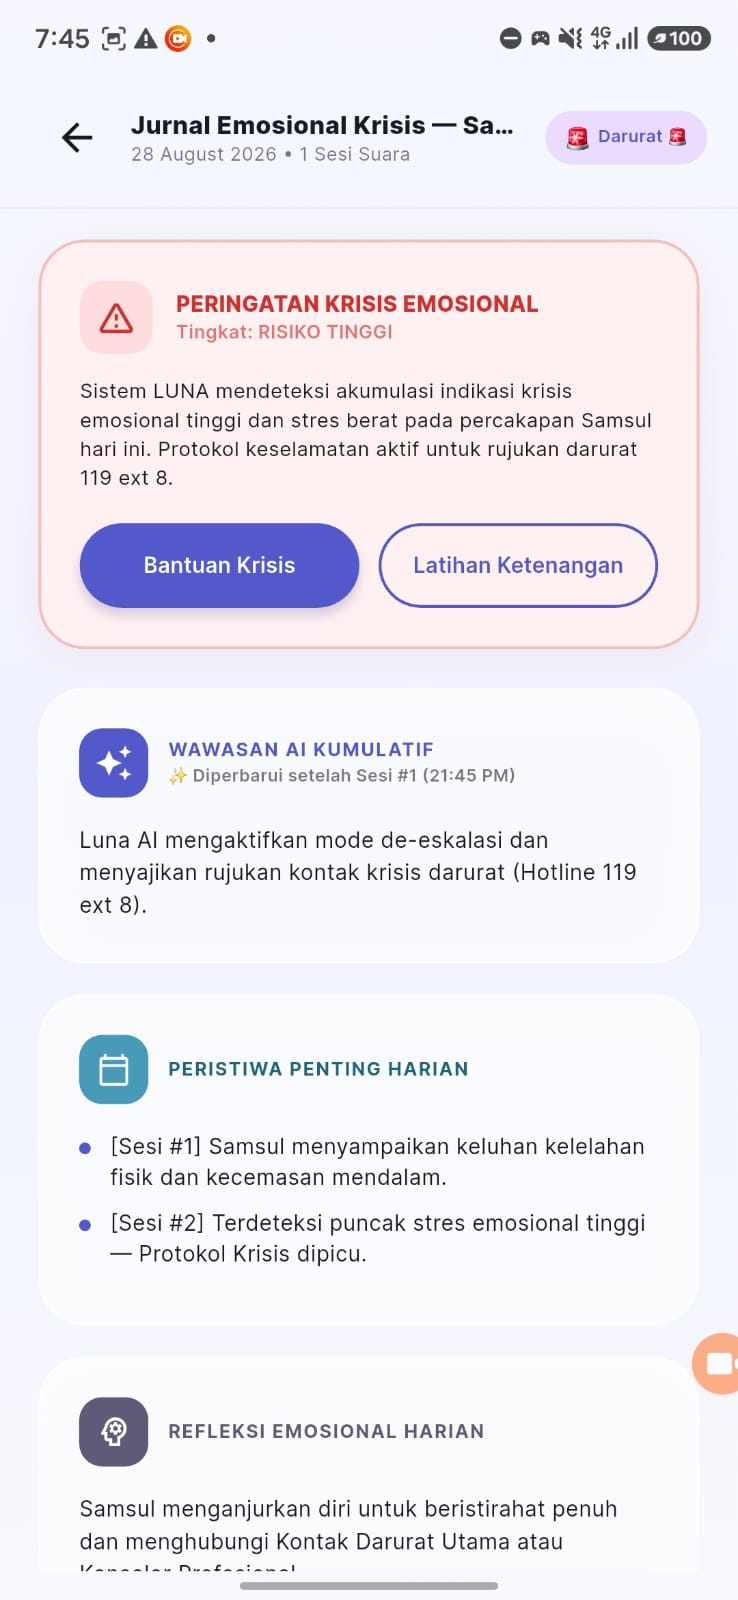
\includegraphics[height=5.8cm,keepaspectratio]{images/prototype/journal_detail_crisis.jpeg}
            };
        \end{tikzpicture}\\[0.3em]
        {\small\itshape (b) Detail Rekomendasi \& Intervensi}
    \end{minipage}
    \vspace{0.2em}
    \caption{Personalized Recommendation}
\end{figure}

\subsubsecstyle{j. Support \& Emergency}
\begin{figure}[H]
    \centering
    \begin{minipage}[b]{0.45\textwidth}
        \centering
        \begin{tikzpicture}
            \node[
                draw=TealAccent,
                fill=white,
                line width=0.8pt,
                rounded corners=6pt,
                inner sep=2pt
            ] {
                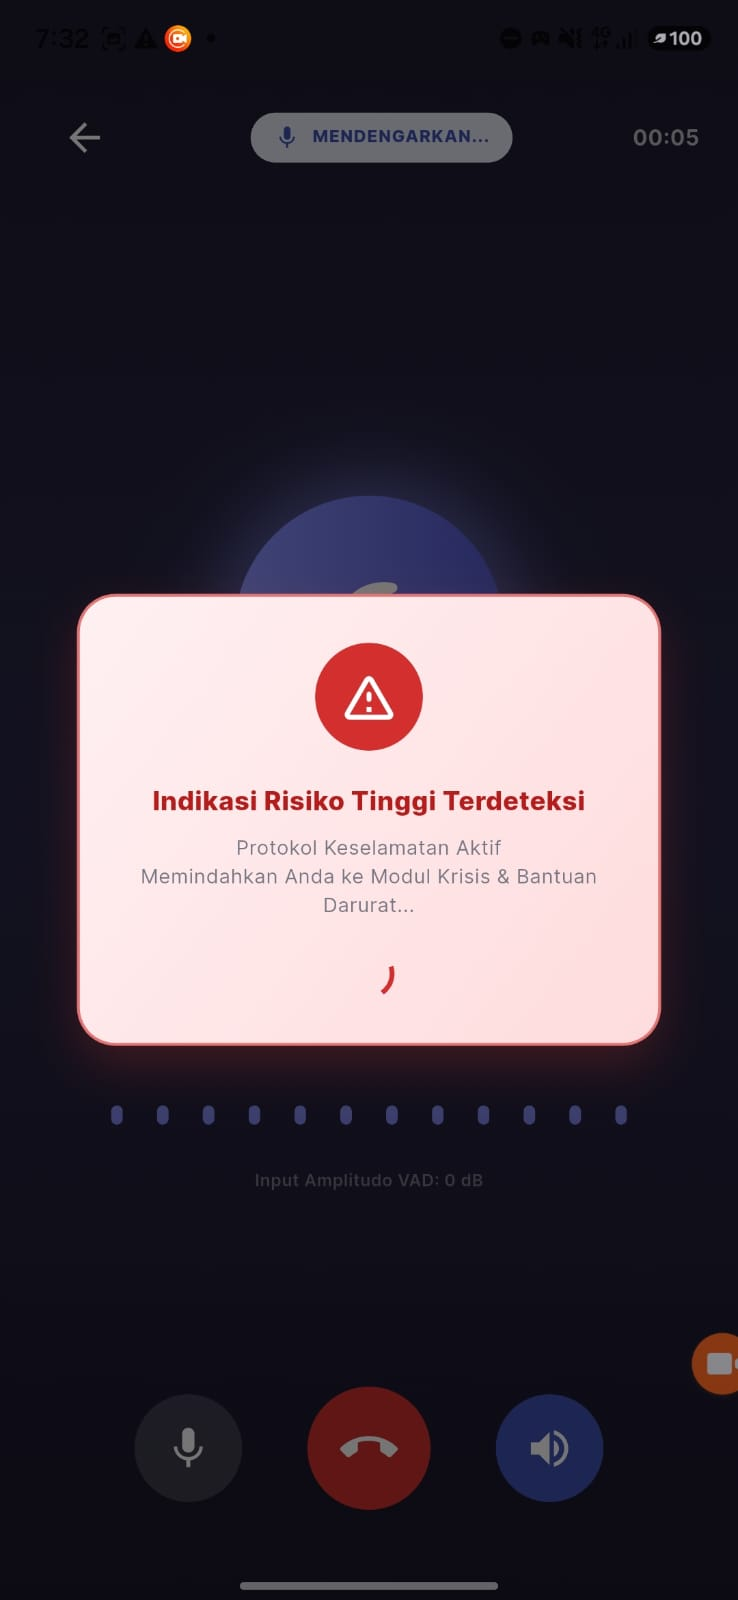
\includegraphics[height=5.8cm,keepaspectratio]{images/prototype/crisis_alert_dialog.jpeg}
            };
        \end{tikzpicture}\\[0.3em]
        {\small\itshape (a) Pop-up Peringatan High Risk}
    \end{minipage}%
    \hfill
    \begin{minipage}[b]{0.45\textwidth}
        \centering
        \begin{tikzpicture}
            \node[
                draw=TealAccent,
                fill=white,
                line width=0.8pt,
                rounded corners=6pt,
                inner sep=2pt
            ] {
                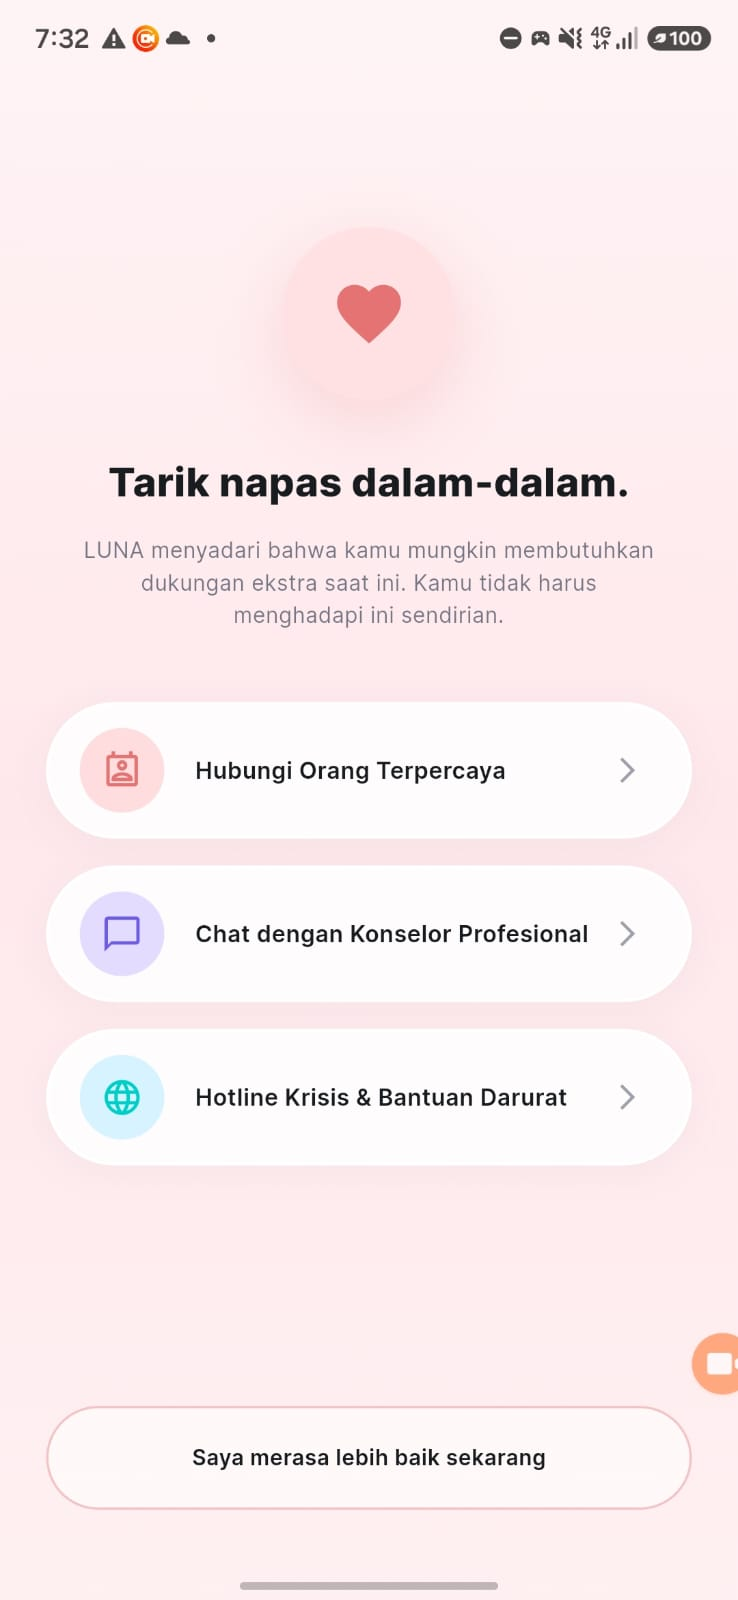
\includegraphics[height=5.8cm,keepaspectratio]{images/prototype/crisis_module_screen.jpeg}
            };
        \end{tikzpicture}\\[0.3em]
        {\small\itshape (b) Layar Modul Krisis \& Support Hotline}
    \end{minipage}
    \vspace{0.2em}
    \caption{Support \& Emergency}
\end{figure}

\clearpage
\lampiranhead{5. Dokumentasi Penggunaan}

\subsubsecstyle{a. Membuka Aplikasi}
\noindent\textbf{Tujuan:} Masuk ke halaman utama LUNA (Gambar 9, 10).\par
\noindent\textbf{Langkah:}
\begin{enumerate}[leftmargin=1.5em,label=\arabic*.,itemsep=2pt,topsep=2pt]
    \item Buka aplikasi LUNA.
    \item Pilih Login atau Daftar.
    \item Masuk ke Home.
\end{enumerate}

\subsubsecstyle{b. Memulai Percakapan AI}
\noindent\textbf{Tujuan:} Memulai sesi konsultasi (Gambar 13).\par
\noindent\textbf{Langkah:}
\begin{enumerate}[leftmargin=1.5em,label=\arabic*.,itemsep=2pt,topsep=2pt]
    \item Tekan menu AI Conversation.
    \item Ketik pesan atau gunakan mikrofon.
    \item AI mulai merespons.
\end{enumerate}

\subsubsecstyle{c. Voice Conversation}
\noindent\textbf{Tujuan:} Melakukan percakapan suara (Gambar 14).\par
\noindent\textbf{Langkah:}
\begin{enumerate}[leftmargin=1.5em,label=\arabic*.,itemsep=2pt,topsep=2pt]
    \item Tekan tombol Voice.
    \item Izinkan akses mikrofon.
    \item Mulai berbicara.
    \item AI memberikan respons suara.
\end{enumerate}

\subsubsecstyle{d. AI Diary}
\noindent\textbf{Tujuan:} Melihat diary otomatis (Gambar 15).\par
\noindent\textbf{Langkah:}
\begin{enumerate}[leftmargin=1.5em,label=\arabic*.,itemsep=2pt,topsep=2pt]
    \item Buka menu Diary.
    \item Pilih tanggal.
    \item Sistem menampilkan ringkasan percakapan.
\end{enumerate}

\subsubsecstyle{e. Monitoring}
\noindent\textbf{Tujuan:} Melihat perkembangan kondisi mental (Gambar 16).\par
\noindent\textbf{Langkah:}
\begin{enumerate}[leftmargin=1.5em,label=\arabic*.,itemsep=2pt,topsep=2pt]
    \item Pilih menu Monitoring.
    \item Sistem menampilkan grafik emosi.
    \item Lihat perubahan kondisi dari waktu ke waktu.
\end{enumerate}

\subsubsecstyle{f. Recommendation}
\noindent\textbf{Tujuan:} Melihat rekomendasi personal (Gambar 17).\par
\noindent\textbf{Langkah:}
\begin{enumerate}[leftmargin=1.5em,label=\arabic*.,itemsep=2pt,topsep=2pt]
    \item Buka Recommendation.
    \item Sistem menampilkan aktivitas yang direkomendasikan.
    \item Pengguna dapat menandai aktivitas sebagai selesai.
\end{enumerate}

\subsubsecstyle{g. Support}
\noindent\textbf{Tujuan:} Mengakses bantuan ketika diperlukan (Gambar 18).\par
\noindent\textbf{Langkah:}
\begin{enumerate}[leftmargin=1.5em,label=\arabic*.,itemsep=2pt,topsep=2pt]
    \item Pilih menu Support.
    \item Sistem menampilkan informasi bantuan.
    \item Jika diperlukan, sistem memberikan arahan sesuai tingkat risiko.
\end{enumerate}

\clearpage
\lampiranhead{6. Bukti Wawancara Psikolog (Studi Pendahuluan DASS-21 \& Rencana Uji Coba)}

\indent Dokumentasi wawancara klinis dan konsultasi ilmiah bersama \textbf{Qori Fanani, M.Psi., Psikolog} (Petugas Poliklinik Politeknik Negeri Malang dan Dosen Psikologi Universitas Kepanjen) mengenai validasi kerangka kerja instrumen DASS-21 (\textit{Depression Anxiety Stress Scale 21}) serta penjajakan kerja sama \textit{clinical trial} aplikasi LUNA disajikan pada Gambar 19.

\indent Melalui diskusi ini, pakar mengonfirmasi validitas pembagian tingkat keparahan distres mental pengguna menjadi Level 1 (\textit{Mild}), Level 2 (\textit{Moderate}), dan Level 3 (\textit{Severe/Extremely Severe}) yang diterapkan pada mesin pemicu intervensi LUNA. Selain itu, pihak Poliklinik Polinema menyambut baik dan sangat terbuka terhadap pelaksanaan \textit{pilot testing} dan uji coba klinis penggunaan LUNA pada mahasiswa maupun pasien Poliklinik Polinema sebagai bagian dari peta jalan evaluasi efektivitas sistem.

\begin{figure}[H]
    \centering
    \begin{tikzpicture}
        \node[
            draw=TealAccent,
            fill=white,
            line width=0.8pt,
            rounded corners=6pt,
            inner sep=2pt
        ] {
            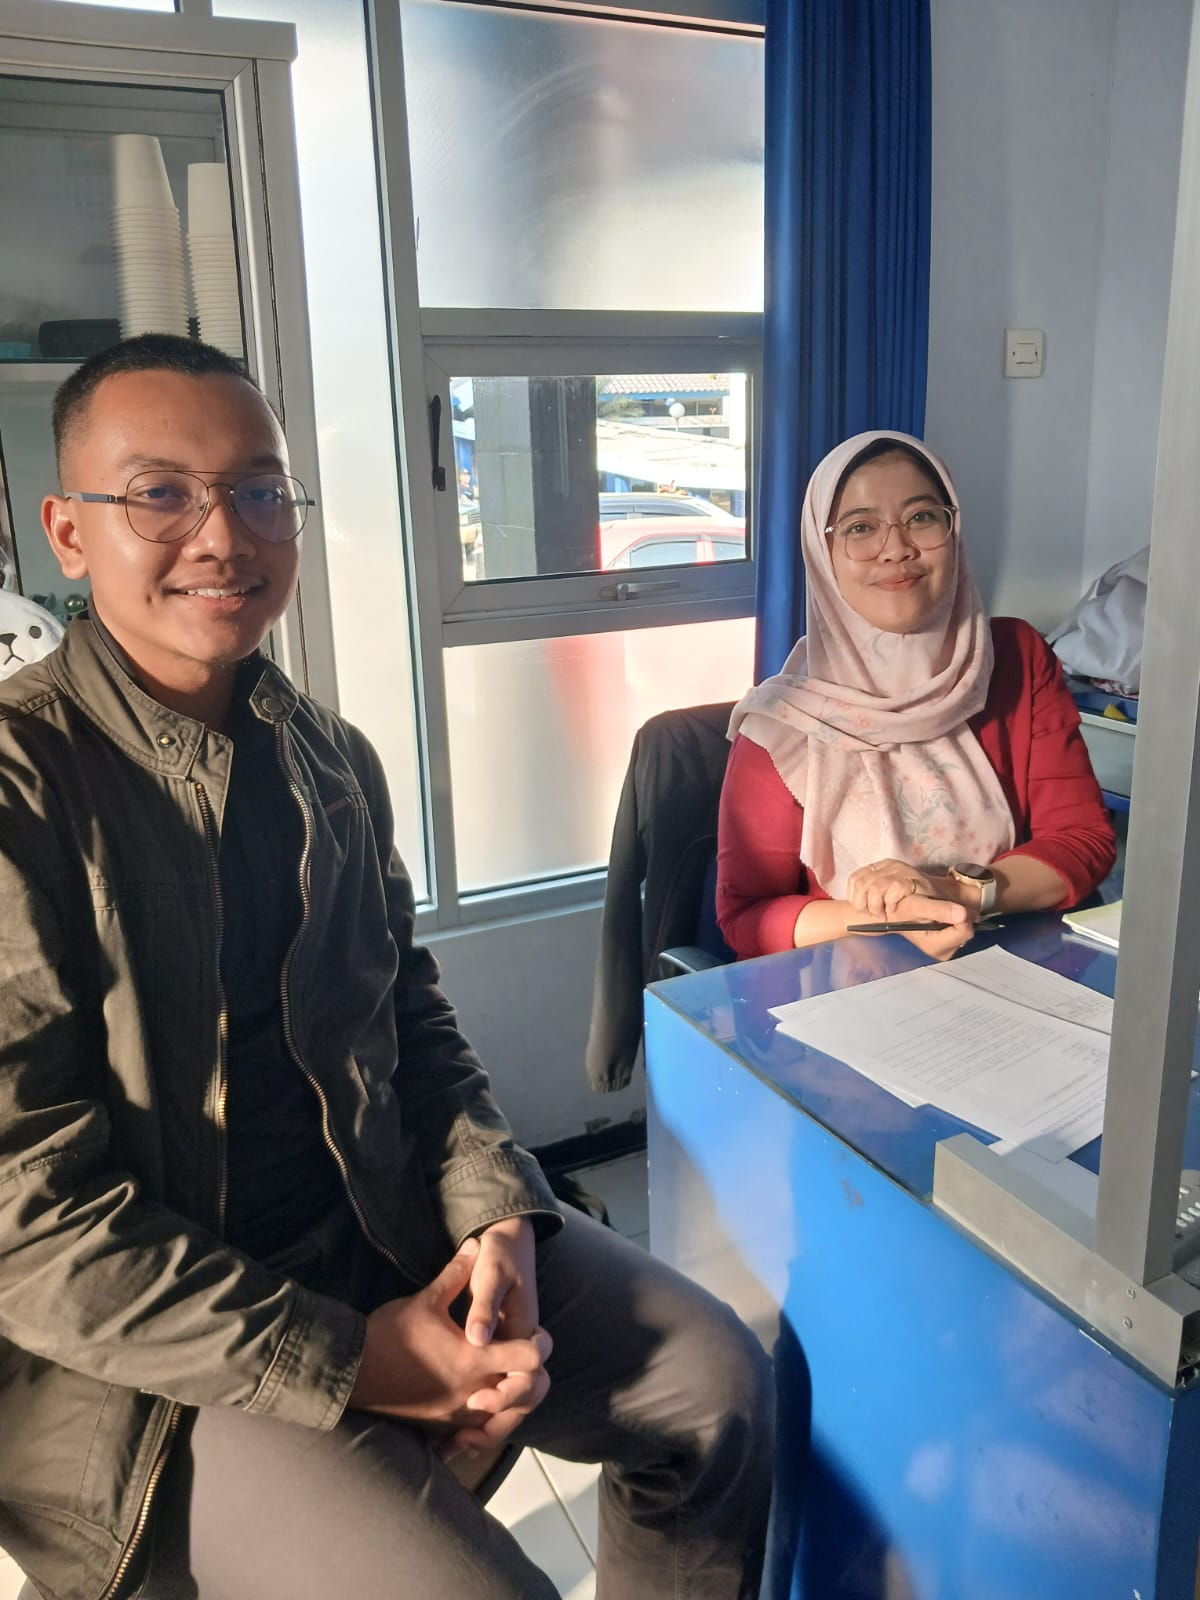
\includegraphics[height=12.5cm,keepaspectratio]{images/lampiran/fig9_wawancara_psikolog.png}
        };
    \end{tikzpicture}
    \caption{Dokumentasi Wawancara dengan Qori Fanani, M.Psi., Psikolog}
\end{figure}

\clearpage
\lampiranhead{7. Surat Pernyataan Orisinalitas Karya}

\begin{figure}[H]
    \centering
    \begin{tikzpicture}
        \node[
            draw=TealAccent,
            fill=white,
            line width=0.8pt,
            rounded corners=6pt,
            inner sep=2pt
        ] {
            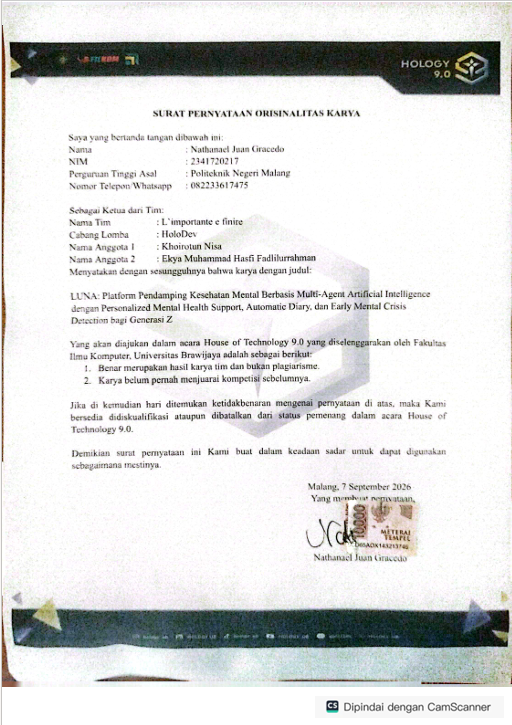
\includegraphics[width=0.88\textwidth,keepaspectratio]{images/surat pernyataan.png}
        };
    \end{tikzpicture}
    \caption{Surat Pernyataan Orisinalitas Karya (Ber-meterai \& Ditandatangani)}
\end{figure}

\clearpage
\lampiranhead{8. Tautan Video Demo Aplikasi \& Berkas Akses}

\indent Sebagai pemenuhan persyaratan kompetisi HoloDev HOLOGY 9.0, berikut adalah daftar tautan akses publik untuk video pengujian demo perangkat lunak dan repositori berkas implementasi:

\begin{enumerate}[leftmargin=*,label=\arabic*.,itemsep=0.5em]
    \item \textbf{Tautan Video Demo Aplikasi (Google Drive):}\\
    \url{https://drive.google.com/file/d/1leySp4r29Kz3TLDlhNC1YP4iOxChis1a/view?usp=drive_link}\\
    {\small\itshape (Video berdurasi $\le$ 10 menit berisi pengenalan tim, latar belakang solusi, serta peragaan fungsionalitas utama aplikasi LUNA).}
    
    \item \textbf{Tautan Google Drive Berkas Source Code, Build APK \& Dokumentasi:}\\
    \url{https://drive.google.com/drive/folders/1bJp6CdtFBXfh3RJ8tv2wlBQT3z1xdhio?usp=drive_link}\\
    {\small\itshape (Berisi berkas build APK/Web, source code backend FastAPI, FastMCP tools, dan kode aplikasi Flutter luna\_mobile).}
\end{enumerate}



\end{document}
